% Chapter ?

\chapter{Algorithms} % Main chapter title
\label{algo} % For referencing the chapter elsewhere, use \ref{Chapter1} 

\lhead{Chapter 3. \emph{Algorithms}} % This is for the header on each page - perhaps a shortened title



%%%%%%%%%%%%%%%%%%%%%%%%%%%%%%%%%
%%% Commands used in the text %%%
%%%%%%%%%%%%%%%%%%%%%%%%%%%%%%%%%

\newcommand{\maxerror}{\textit{$\epsilon$}}
\newcommand{\maskalgo}{\textit{M}}
\newcommand{\NOmaskalgo}{\textit{NM}}
\newcommand{\intCoder}{\textit{algo\_key}}
\newcommand{\win}{\textit{w}}
\newcommand{\nodata}{\textit{NO\_DATA}}
\newcommand{\nodatafloat}{\textit{NO\_DATA\_FLOAT}}
\newcommand{\colSize}{\textit{col\_size}}
\newcommand{\sizee}{\textit{size}}
\newcommand{\noData}{\textnormal{``N"}}
\newcommand{\logWinSize}{\ceil{\log _{2} \win}}
\newcommand{\logWinSizeOpt}[1]{\log _{2} {#1}}

% APCA
\newcommand{\midrange}{\textit{mid\_range}}
\newcommand{\incoming}{\textit{E}}
\newcommand{\point}{$\incoming$}
% FR
\newcommand{\disPoints}{\textit{displaced\_points}}
\newcommand{\getDisplacedPointsMethod}{\textnormal{GetDisplacedPoints}}
\newcommand{\firstIndex}{\textit{i}_o}
\newcommand{\lastIndex}{\textit{i}_f}
\newcommand{\pointi}{$P_{i}$}
\newcommand{\pointo}{$P_{o}$}
\newcommand{\pointf}{$P_{f}$}
\newcommand{\half}{\textit{half}}
\newcommand{\decodeSegment}{\textnormal{DecodeSegment}}
\newcommand{\segment}{\textit{segment}}
\newcommand{\validSegment}{\textit{valid\_segment}}

% CA
\newcommand{\archived}{\textit{A}}
\newcommand{\incomingP}[1]{\textit{E{#1}}}
\newcommand{\snapshot}{\textit{S}}
\newcommand{\smax}{\textit{SMax}}
\newcommand{\smaxo}{\textit{SMaxOld}}
\newcommand{\smin}{\textit{SMin}}
\newcommand{\smino}{\textit{SMinOld}}
\newcommand{\EseE}{\textit{SE}}
\newcommand{\EseEP}[1]{\textit{SE{#1}}}

% GAMPS
\newcommand{\epsilonB}{\textit{$\epsilon_b$}}
\newcommand{\epsilonR}{\textit{$\epsilon_r$}}
\newcommand{\columns}{\textit{columns}}

% SF
\newcommand{\segmentSet}{\textit{LS}}
\newcommand{\segmentLast}{\segment_{\textit{prev}}}
\newcommand{\connected}{\textit{connected}}
\newcommand{\pointO}{\textit{P}_{\textit{o}}}
\newcommand{\pointF}{\textit{P}_{\textit{f}}}



\newcommand{\beginAlgorithm}{
    \setlength{\algomargin}{1em}
    \IncMargin{1em}
    \begin{figure}[ht]
    \begin{algorithm}[H]
    
    \SetAlgoLined
    \SetKwInOut{Input}{input}
    \SetKwInOut{Output}{output}
}

\newcommand{\onlyInput}[1]{
    \Indm  
    \SetAlgoLined
    \Input{#1}
    \Indp
}

\newcommand{\onlyOutput}[1]{
    \Indm  
    \SetAlgoLined
    \Output{#1}
    \Indp
}

\newcommand{\inputAndOutput}[2]{
    \Indm  
    \SetAlgoLined
    \Input{#1}
    \Output{#2}
    \Indp
}


\newcommand{\EndPseudo}[2]{
    \end{algorithm}
    \vspace{-15pt}
    \caption{{#1}}
    {#2}
    \end{figure}
}

% TODO: remove
\newcommand{\EndAlgorithm}[2]{
    \EndPseudo{{#1} pseudocode. TODO: remove}{{#2}}
}

\newcommand{\EndAlgorithmTwo}[3]{
    \EndPseudo{{#1} routine for algorithm {#2}.}{{#3}}
}

\newcommand{\EndAlgorithmVariant}[4]{
    \EndPseudo{{#1} routine for variant {#3} of algorithm {#2}.}{{#4}}
}

% https://tex.stackexchange.com/a/461831
\SetKwFor{RepTimes}{repeat}{times}{end}


\newcommand{\eqqq}{$ == $}
\newcommand{\difff}{$ != $}
\newcommand{\orr}{\ \textbf{\upshape or}\ }
\newcommand{\andd}{\ \textbf{\upshape and}\ }
\newcommand{\truee}{\textbf{\upshape true}\ }
\newcommand{\continueAlgo}{\textbf{continue}}
\newcommand{\notCond}{\textnormal{\textbf{not}}}
\newcommand{\nott}{\textnormal{\textbf{not}}}
\newcommand{\breakAlgo}{\textbf{break}}
\newcommand{\returnn}{\textbf{return }}
\newcommand{\commaa}{\textnormal{,}}


\newcommand{\coderBase}{\text{Base}}
\newcommand{\coderPCA}{\text{PCA}}
\newcommand{\coderAPCA}{\text{APCA}}
\newcommand{\coderCA}{\text{CA}}
\newcommand{\coderPWLH}{\text{PWLH}}
\newcommand{\coderPWLHInt}{\text{PWLHInt}}
\newcommand{\coderFR}{\text{FR}}
\newcommand{\coderSF}{\text{SF}}
\newcommand{\coderGAMPS}{\text{GAMPS}}


%%%%%%%%%%%%%%%%%%%%%%%%%%%%%%%%
%% CODER AND DECODER COMMANDS %%
%%%%%%%%%%%%%%%%%%%%%%%%%%%%%%%%
\newcommand{\minn}{\textit{min}}
\newcommand{\maxx}{\textit{max}}
\newcommand{\error}{\textit{err}}
\newcommand{\file}{\textit{in}}
\newcommand{\out}{\textit{out}}
\newcommand{\window}{\textit{win}}
\newcommand{\arrayy}{\textit{array}}
\newcommand{\windowVal}{\textit{win\_val}}
\newcommand{\windowSize}{$\textnormal{|}\window\textnormal{|}$}
\newcommand{\windowSizeT}{|\window|}

\newcommand{\encodedColumn}{\textit{encoded\_column}}
\newcommand{\entry}{\textit{entry}}
\newcommand{\valuev}{\textit{value}}
\newcommand{\binFile}{binary file}
\newcommand{\variant}{\textit{v}}

%%%%%%%%%%%%%%%%%%%%%%%%%%%%%%%%
%% CODER COMMANDS %%%%%%%%%%%%%%
%%%%%%%%%%%%%%%%%%%%%%%%%%%%%%%%
\newcommand{\cInputFile}{\file: csv data file to be encoded}
\newcommand{\cInputColSize}{\colSize: number of entries in the column}

\newcommand{\cOutputFileA}{\out: \binFile \ with the encoding of \file}
\newcommand{\cOutputFile}[1]{\out: \binFile\ encoded with algorithm #1}


\newcommand{\forEachEntryCoder}{\textnormal{entry in} \column\commaa\ \entry\commaa}

\newcommand{\createWindow}{Create an empty window, \window}
\newcommand{\createWindoww}{create an empty window, \window}
\newcommand{\windowNotFullOne}{$\windowSize < \win$}
\newcommand{\windowNotFullTwo}{$\windowSize \leq \win$}
\newcommand{\windowFull}{$\windowSize \eqqq \win$}
\newcommand{\validThreTwo}{$|\maxx - \minn| \leq 2*\maxerror$}

\newcommand{\ifNoDataCoder}[1]{${#1} \eqqq \noData$\xspace}

%%%%%%%%%%%%%%%%%%%%%%%%%%%%%%%%
%% DECODER COMMANDS %%%%%%%%%%%%
%%%%%%%%%%%%%%%%%%%%%%%%%%%%%%%%

\newcommand{\dinputCol}[1]{\column: column encoded with algorithm #1}
\newcommand{\dinputfileA}{\file: coded \binFile}
\newcommand{\dinputfile}[1]{\file: \binFile\ coded with algorithm #1}
\newcommand{\doutputfile}{\out: decoded csv data file}

\newcommand{\cInputVariant}{\variant: variant (\maskalgo\ or \NOmaskalgo)}
\newcommand{\cInputThreshold}{\maxerror: maximum error threshold}
\newcommand{\cInputWindow}{\win: window size}
\newcommand{\cInputThresholdOpt}{\cInputThreshold} %\ // ignored by algorithm Base}
\newcommand{\cInputWindowOpt}{\cInputWindow} % \ // ignored by algorithms Base and SF}

\newcommand{\tsColumn}{\text{ts\_column}}
\newcommand{\maskModeNoS}{$\variant \eqqq \maskalgo$}
\newcommand{\maskMode}{\maskModeNoS\ }

\newcommand{\whileColumnLeftToDecode}{$\notCond\ \file.\textnormal{column\_decoded?}$}
\newcommand{\whileColumnNotDecoded}{$n < \colSize$}

%%%%%%%%%%%%%%%%%%%%%%%%%%%%%%%%%%%%%%%%%%%%%%%%%%%%%%%%%%%%%%%%
%%%%%%%%%%%%%%%%%%%%%%%%%%%%%%%%%%%%%%%%%%%%%%%%%%%%%%%%%%%%%%%%

\newcommand{\commonSpecific}[2]{{#1} {#2} using a (column-specific) fixed number of bits}
\newcommand{\encodeSpecific}[1]{\commonSpecific{Encode}{{#1}}}
\newcommand{\decodeSpecific}[1]{\commonSpecific{Decode}{{#1}}}

\newcommand{\codeFloat}[1]{Encode {#1} as a float, using 32 bits}
\newcommand{\decodeFloat}[1]{Decode {#1} as a float, using 32 bits}

\newcommand{\calculateMinMax}{Let \minn\ and \maxx\ be the minimum and maximum sample values in \window}
\newcommand{\recalculateMinMax}{recalculate \minn\ and \maxx}

\newcommand{\encodeWindowSize}{Encode $\windowSize$ using $\logWinSize$ bits}
\newcommand{\decodeWindowwSize}{Decode $\sizee$ using $\logWinSize$ bits}


%% BASE - CODER
\newcommand{\columnInput}{\column: column of the csv data file to be encoded}

%% PCA - CODER
\newcommand{\cInputWindowPCA}{\win: fixed window size}
\newcommand{\calculateMidrange}{$\midrange = (\windowMin + \windowMax)/2$}
\newcommand{\calculateMidrangeTwo}{$\midrange = (\minn + \maxx)/2$}
\newcommand{\codeMidrange}{\codeInt(\midrange, \colTotBits)}
\newcommand{\eachValueInWindow}{\textnormal{sample in} \window\commaa\ \valuev,}
\newcommand{\eachEntryInWindow}{\textnormal{entry in} \window\commaa\ \entry,}
\newcommand{\codeBit}[1]{Output bit {#1} to \out}
%% PCA - DECODER
\newcommand{\nEqZero}{$n = 0$}
\newcommand{\calculateSize}{$\sizee = \min\{\win, \colSize - n\}$}
\newcommand{\decodeValuePCA}{\decodeSpecific{\midrange}}
\newcommand{\addNToSize}{$n \mathrel{+}= \sizee$}
\newcommand{\bit}{\textit{bit}}
\newcommand{\decodeBit}{Decode \bit\ from \file}

%% APCA - CODER
\newcommand{\cInputWindowAPCA}{\win: maximum window size}
\newcommand{\codeWindowValue}{\codeInt(\windowCodeValue, \colTotBits)}
\newcommand{\updateMinMaxx}{Let $m  = \min \{\minn, \entry\}$ and $M  = \max \{\maxx, \entry\}$}
\newcommand{\NOTvalidThreThree}{$(M - m) > 2*\maxerror$}
\newcommand{\encodeWindowAPCA}{EncodeWindow(\window, \out, \win) // routine shown in Figure~\ref{apcaWindowM}}
\newcommand{\AddEntry}{Add \entry\ to \window}
%% APCA - WIN
\newcommand{\windowInput}{\window: window to encode}
\newcommand{\encodeWindowSizee}{Encode $|\window|$ using $\logWinSize$ bits}
\newcommand{\encodeWindowSizeeOne}{Encode 1 using $\logWinSize$ bits}

%% DECO - LINEAR
\newcommand{\tss}{\textit{t}}
\newcommand{\sv}{\textit{s}}
\newcommand{\tscol}{\textit{t\_col}}
\newcommand{\tsO}{$\tss_o$}
\newcommand{\tsN}{$\tss_f$}
\newcommand{\tsI}{$\tss_i$}
\newcommand{\sO}{$\sv_o$}
\newcommand{\sN}{$\sv_f$}
\newcommand{\sI}{$\sv_i$}

\newcommand{\inputTSCol}{\tscol: timestamps column}
\newcommand{\inputTSO}{\tsO: timestamp of the first endpoint of the segment}
\newcommand{\inputTSN}{\tsN: timestamp of the last endpoint of the segment}
\newcommand{\inputSO}{\sO: sample value of the first endpoint of the segment}
\newcommand{\inputSN}{\sN: sample value of the last endpoint of the segment}

\newcommand{\decodedSamples}{\textit{decoded\_samples}}
\newcommand{\decodedSamplesTwo}{\textit{samples}}
\newcommand{\outputDecoded}{\decodedSamples: list with the sample values decoded from the segment}
\newcommand{\forEachTS}{\textnormal{timestamp in \tscol,} \tsI,}
\newcommand{\ifDecoLinear}{\tsO \ $\leq$ \tsI \ $\leq$ \tsN}
\newcommand{\AddEntryLinear}{Add \sI\ to \decodedSamples}


\newcommand{\exampleFigure}[5]{
\begin{figure}[{#5}]
\begin{center}
\hspace*{-0.08\textwidth}
\includegraphics[clip, trim=0cm 0cm 0cm 0.85cm, width=1.1\textwidth]{chapters/3-Algorithms/examples/#1/#1#2.pdf}
\vspace{-25pt}
\caption{{#4}}
{#3}
\end{center}
\end{figure}
}

\newcommand{\exampleStepCommon}[4]{
\exampleFigure{#1}{#2}{#3}{#4}{h}
}

\newcommand{\makeCaption}[4]{Example: Algorithm variant \MaskVar{\uppercase{#1}} with $\maxerror={#2}$ and $\win={#3}$. Step {#4}.}

\newcommand{\commonIntro}[4]{Example: {#4}. Variant \MaskVar{\uppercase{#1}} with $\maxerror={#2}$. Step~{#3}.}
\newcommand{\makeCaptionIntroPWLH}[3]{\commonIntro{#1}{#2}{#3}{checking the valid hull condition}}
\newcommand{\makeCaptionIntroCA}[3]{\commonIntro{#1}{#2}{#3}{key steps of the coding algorithm}}
\newcommand{\makeCaptionIntroSF}[3]{\commonIntro{#1}{#2}{#3}{key steps of the coding algorithm}}


\newcommand{\exampleStepPCA}[4]{
\exampleStepCommon{#1}{#2}{#3}{\makeCaption{#1}{1}{4}{#4}}
}

\newcommand{\exampleStepGAMPS}[4]{
\exampleStepCommon{#1}{#2}{#3}{\makeCaption{#1}{0}{256}{#4}}
}

\newcommand{\exampleStep}[4]{
\exampleStepCommon{#1}{#2}{#3}{\makeCaption{#1}{1}{256}{#4}}
}

\newcommand{\exampleStepMany}[4]{
\exampleFigure{#1}{#2}{#3}{\makeCaption{#1}{1}{256}{#4}}{H}
}


%%%%%%%%%%%%%%%%%%%%%%%%%%%%%%%%%%%%%%%%%%%%%%%%%%%%%
%%%%%%%%%%%%%%%%%%%%%%%%%%%%%%%%%%%%%%%%%%%%%%%%%%%%%
%%%%%%%%%%%%%%%%%%%%%%%%%%%%%%%%%%%%%%%%%%%%%%%%%%%%%

\newcommand{\examplelinear}{
\centering
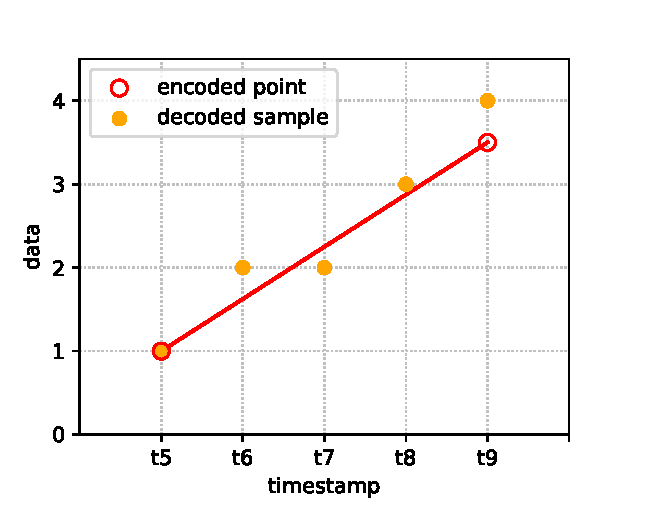
\includegraphics[width=1.2\textwidth]{chapters/3-Algorithms/examples/linear.pdf}
\vspace{-5pt}
\begin{minipage}{1.17\textwidth}
\captionof{figure}{Example of the auxiliary routine \decodeSegment\ for linear model algorithms.}
% \captionof{figure}{Example: auxiliary routine \decodeSegment\ for linear model algorithms.}
\label{example:linear}
\end{minipage}
}

\newcommand{\examplePWLH}{
\begin{figure}[h]
% \centering
\hspace{-30pt}
\begin{minipage}{.55\textwidth}
  \centering
  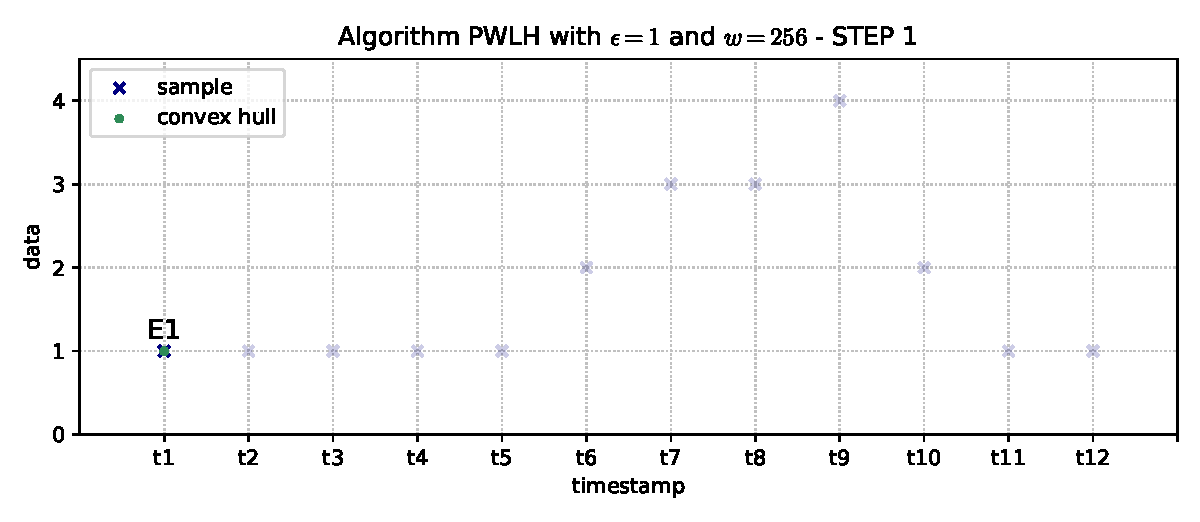
\includegraphics[clip, trim=0cm 0cm 0cm 0.9cm,width=1.0\linewidth]{chapters/3-Algorithms/examples/pwlh_intro/pwlh1.pdf}
  \vspace{-25pt}
  \captionof{figure}{\makeCaptionIntroPWLH{pwlh}{1}{1}}
  \label{example:pwlhIntro1}
\end{minipage}
\begin{minipage}{.55\textwidth}
  \centering
  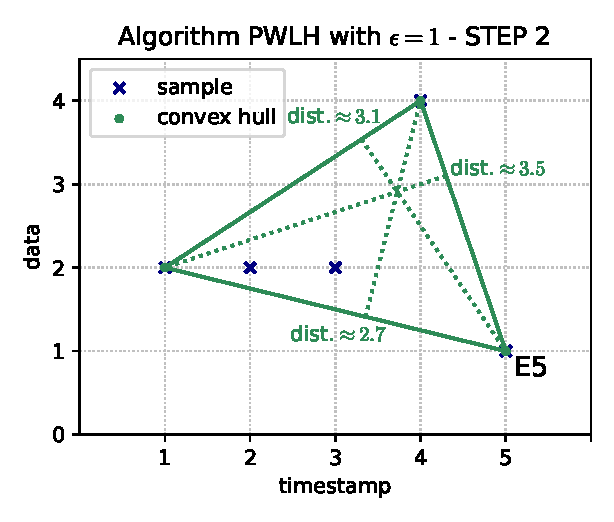
\includegraphics[clip, trim=0cm 0cm 0cm 0.9cm,width=1.0\linewidth]{chapters/3-Algorithms/examples/pwlh_intro/pwlh2.pdf}
  \vspace{-25pt}
  \captionof{figure}{\makeCaptionIntroPWLH{pwlh}{1}{2}}
  \label{example:pwlhIntro2}
\end{minipage}
\end{figure}
}

\newcommand{\exampleCA}{
\begin{figure}[h]
% \centering
\hspace{-30pt}
\begin{minipage}{.55\textwidth}
  \centering
  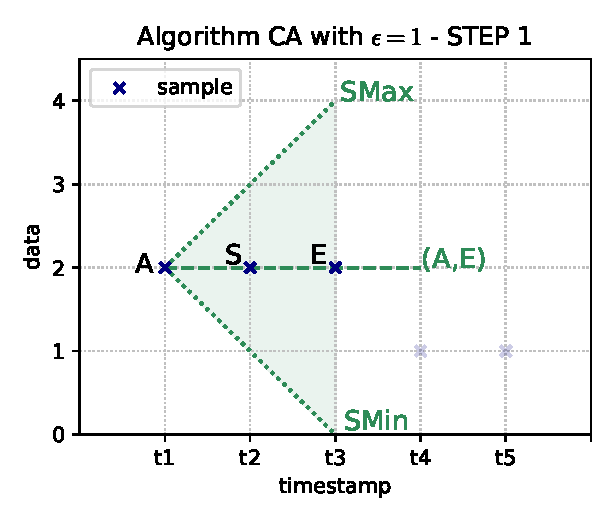
\includegraphics[clip, trim=0cm 0cm 0cm 0.9cm,width=1.0\linewidth]{chapters/3-Algorithms/examples/ca_intro/ca1.pdf}
  \vspace{-25pt}
  \captionof{figure}{\makeCaptionIntroCA{ca}{1}{1}}
  \label{example:caIntro1}
\end{minipage}%
\begin{minipage}{.55\textwidth}
  \centering
  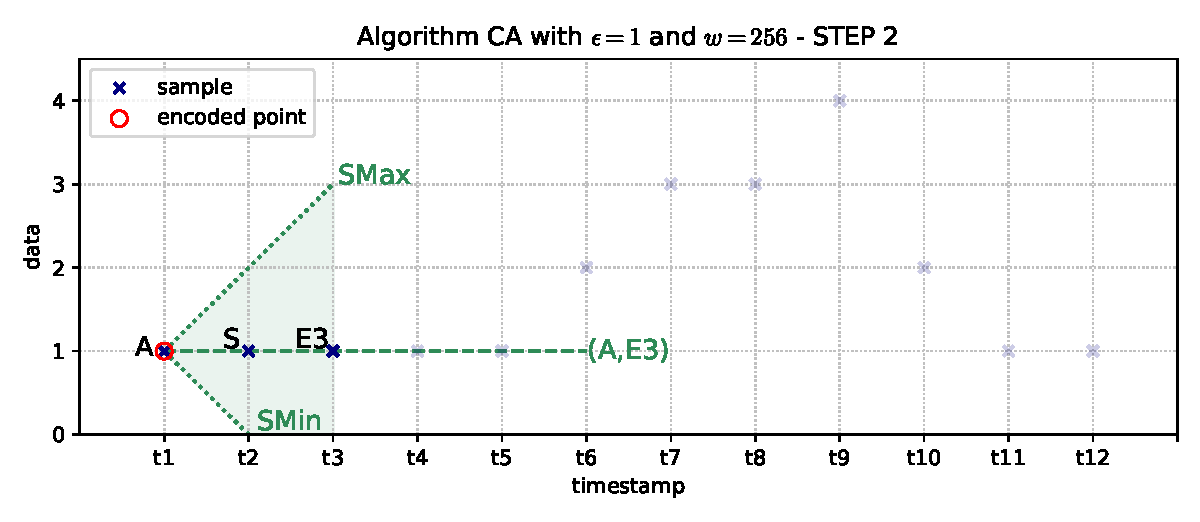
\includegraphics[clip, trim=0cm 0cm 0cm 0.9cm,width=1.0\linewidth]{chapters/3-Algorithms/examples/ca_intro/ca2.pdf}
  \vspace{-25pt}
  \captionof{figure}{\makeCaptionIntroCA{ca}{1}{2}}
  \label{example:caIntro2}
\end{minipage}
\end{figure}
}

\newcommand{\exampleSF}{
\begin{figure}[h]
% \centering
\hspace{-30pt}
\begin{minipage}{.55\textwidth}
  \centering
  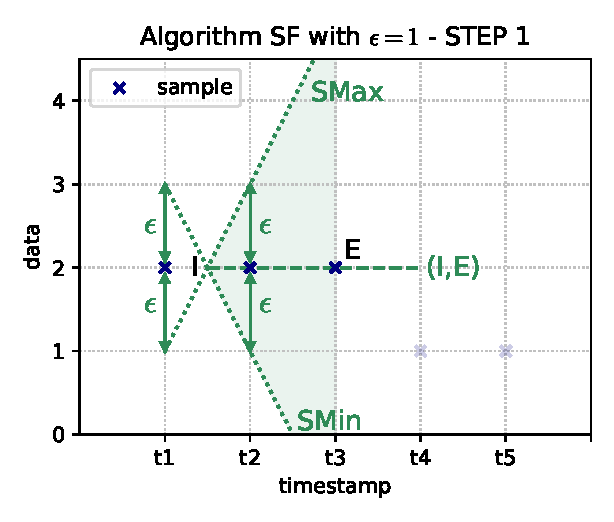
\includegraphics[clip, trim=0cm 0cm 0cm 0.9cm,width=1.0\linewidth]{chapters/3-Algorithms/examples/sf_intro/sf1.pdf}
  \vspace{-25pt}
  \captionof{figure}{\makeCaptionIntroSF{sf}{1}{1}}
  \label{example:sfIntro1}
\end{minipage}%
\begin{minipage}{.55\textwidth}
  \centering
  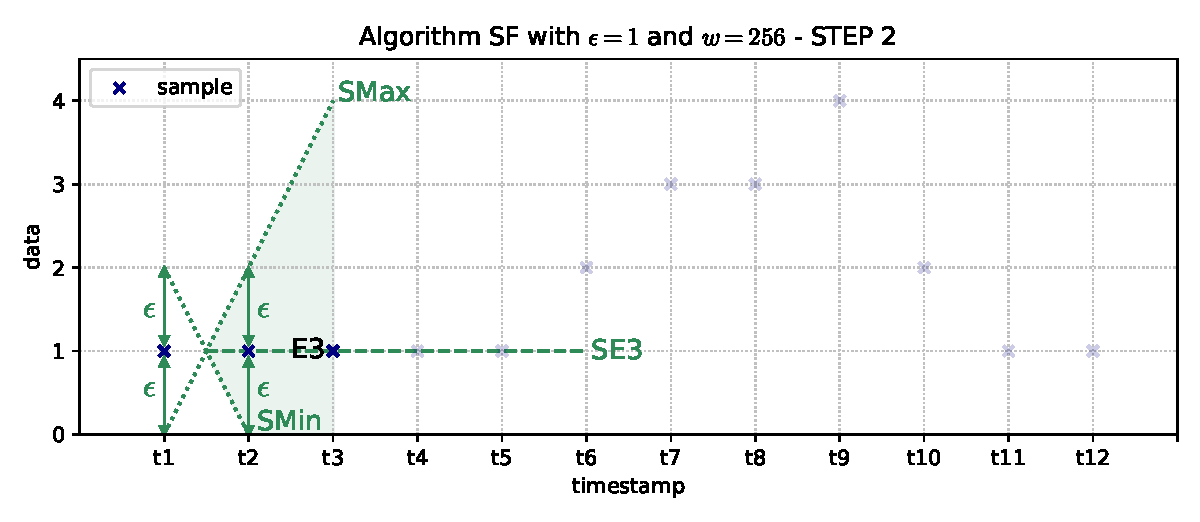
\includegraphics[clip, trim=0cm 0cm 0cm 0.9cm,width=1.0\linewidth]{chapters/3-Algorithms/examples/sf_intro/sf2.pdf}
  \vspace{-25pt}
  \captionof{figure}{\makeCaptionIntroSF{sf}{1}{2}}
  \label{example:sfIntro2}
\end{minipage}
\end{figure}
}







\newcommand{\BeCe}{B_c}


In this chapter we introduce the datasets used in our experiments. Every dataset consists of signals with one or both of the characteristics we are interested in, namely, irregular sampling rate and data gaps. In Chapter~\ref{experiments}, we present our experimental results, which make use of these datasets to analyze the compression performance of our implemented algorithm variants, which are presented in Chapter~\ref{algo}.


The datasets come from multiple sources \dataCite, each using a different data representation format. We transformed the data into a consistent, uniform format, which can be easily adapted to represent different kinds of datasets. In \textbf{Section~\ref{datasets:over}} we describe this format, including an example file that illustrates how the data is represented. In \textbf{sections~\ref{datasets:irkis}} to \textbf{\ref{datasets:wind}} we present each of the eight real-world datasets, namely, IRKIS \cite{dataset:irkis}, SST, ADCP \cite{dataset:sst1}, ElNino \cite{dataset:elnino}, Solar \cite{dataset:solar}, Hail, Tornado, and Wind \cite{dataset:spc}, laying out the source, characteristics and relevant statistics of every signal involved. Finally, in \textbf{Section~\ref{datasets:summary}} we summarize the information presented in this chapter, specifying the number of files, the number of gaps, and the data types of each dataset, as well as the measuring unit, scale, and range of each data type.


\clearpage


\section{Introduction}
\label{algo:overview}


The state-of-the-art algorithms used for sensor data compression reported in the literature \cite{AnEva2013, Signal2016} assume, in general, that the signals have regular sampling and that there are no gaps in the data. However, this is often not true for real-world datasets. For example, all the datasets presented in Chapter~\ref{datasets} consist of signals that miss either one or both of these characteristics. We propose a number of variants of state-of-the-art algorithms, which are able to encode this type of signals. 


We focus on algorithms that support near-lossless compression. Near-lossless compression guarantees a bounded per-sample error between the decompressed and the original signals. The error threshold can be specified by the user via a parameter, denoted~$\maxerror$. Observe that, when $\maxerror$ is equal to 0, compression is lossless, i.e., the decompressed and the original signals are identical.


The algorithms follow a model-based compression approach that compresses signals by exploiting correlation among signal samples taken at close times (\textit{temporal correlation}) and, in some cases, among samples from various signals (\textit{spatial correlation}). In addition to efficient compression performance, they offer some data processing features, like inferring uncertain sensor readings, detecting outliers, indexing, etc. \cite{AnEva2013}. The model-based techniques are classified into different categories, depending on the type of model: \textit{Constant models} approximate signals by piecewise constant functions, \textit{Linear models} use linear functions, and \textit{Correlation models} simultaneously encode multiple signals exploiting temporal and spatial correlation. There also exist \textit{Nonlinear models}, which approximate signals by complex nonlinear functions, but known algorithms that follow this technique do not support near-lossless compression and yield poor compression results~\cite{AnEva2013}. 


For most algorithms we propose two variants, masking (\maskalgo) and non-masking (\NOmaskalgo), which differ in the encoding of the gaps in the data. The \maskalgo\ variant of an algorithm first encodes the position of all the gaps, and then proceeds to encode the data values separately. On the other hand, the \NOmaskalgo\ variant encodes the gaps and the data values simultaneously. Implementation details are presented in the remaining sections of this chapter. We point out that the gaps in a decoded file match the gaps in the original file exactly, regardless of the value of the error threshold parameter (\maxerror). In Section~\ref{secX:rendimiento-relativo} we compare the compression performance of both variants, \maskalgo\ and \NOmaskalgo, for every algorithm that supports both.


Most of the algorithms support a window size parameter, denoted $w$, which defines the size of the blocks into which the data are divided for encoding. In algorithm PCA, parameter $w$ defines a \textit{fixed block size}, while in the rest of the algorithms it defines a \textit{maximum block size}. More details are presented with the specific description of each algorithm, later in this chapter.


In Table~\ref{algo:table:overview} we outline some characteristics of the evaluated algorithms and the proposed variants. For each algorithm, the second and third columns indicate whether it supports lossless and near-lossless compression, respectively, the fourth column shows its model type, the fifth and sixth columns indicate if the masking (\maskalgo) and non-masking (\NOmaskalgo) variants apply, respectively, and the last column specifies if the algorithm depends on a window size parameter ($w$). Algorithm Base is a trivial lossless algorithm that is used as a base ground for comparing the performance of the remaining algorithms, all of which support both lossless and near-lossless encoding.


\clearpage



\begin{table}[h]
\vspace{+5pt}
\begin{center}
    \begin{tabular}{| C{2.2cm} || C{1.4cm} | C{1.4cm} |  C{2cm} |  C{0.9cm} | C{0.9cm} | C{0.7cm} |}
    \hline
      \multicolumn{1}{|>{\centering\arraybackslash}m{2.2cm}||}{\textbf{Algorithm}}
    & \multicolumn{1}{>{\centering\arraybackslash}m{1.4cm}|}{\textbf{Lossless}} 
    & \multicolumn{1}{>{\centering\arraybackslash}m{1.4cm}|}{\textbf{Near-lossless}}
    & \multicolumn{1}{>{\centering\arraybackslash}m{2cm}|}{\textbf{Model}} 
    & \multicolumn{1}{>{\centering\arraybackslash}m{0.9cm}|}{\textbf{\maskalgo}} 
    & \multicolumn{1}{>{\centering\arraybackslash}m{0.9cm}|}{\textbf{\NOmaskalgo}}
    & \multicolumn{1}{>{\centering\arraybackslash}m{0.7cm}|}{\textbf{$w$}}\\
    \hline
    Base                               & x  &   & Constant     &    & x &   \\\hline
    PCA \cite{coder:pca}               & x  & x & Constant     & x  & x & x \\\hline
    APCA \cite{coder:apca}             & x  & x & Constant     & x  & x & x \\\hline
    PWLH \cite{coder:pwlh}/ PWLHInt    & x  & x & Linear       & x  & x & x \\\hline
    CA \cite{coder:ca}                 & x  & x & Linear       & x  & x & x \\\hline
    SF \cite{coder:sf}                 & x  & x & Linear       & x  &   &   \\\hline
    FR \cite{coder:fr}                 & x  & x & Linear       & x  &   & x \\\hline
    GAMPS \cite{coder:gamps}           & x  & x & Correlation  & x  & x & x \\\hline
    \toprule[0.1mm]
    \end{tabular}
    \caption{Characteristics of the evaluated coding algorithms. For each algorithm, the table shows whether it supports lossless and near-lossless compression (second and third columns, respectively), its model type (fourth column), whether the masking (\maskalgo) and non-masking (\NOmaskalgo) variants apply (fifth and sixth columns, respectively), and whether the algorithm depends on a window size parameter ($w$) (last column).}
    \label{algo:table:overview}
\end{center}
\end{table}





% \vspace{-25pt}
\clearpage
\section{General Encoding Scheme}
\label{algo:details}


\vspace{-5pt}
Figure~\ref{pseudoCodeCommon} shows a general encoding scheme used for most of the evaluated algorithms. The decoding scheme is symmetric. Constant and linear model algorithms only exploit the temporal correlation in the data, thus they iterate through the data columns and encode each independently. Since correlation models also exploit the spatial correlation (i.e. the data columns are \textit{not} encoded independently), algorithm GAMPS follows a different scheme, which we present in Section~\ref{algo:gamps}.


In Figure~\ref{pseudoCodeCommon}, the inputs for the coding routine are a CSV data file in the format presented in Chapter~\ref{datasets}, a key ($v$) that describes the algorithm variant (either \maskalgo\ or \NOmaskalgo), and the maximum error threshold (\maxerror) and window size (\win) parameters. The output is a binary file, which represents the input file encoded with a compression algorithm using the specified variant and parameters.


\vspace{+5pt}


\newcommand{\forEachColumnCoder}{\column \textnormal{ in \file.\dataColumns}}

\beginAlgorithm
\inputAndOutput{\cInputFile\\ \cInputVariant\\ \cInputThresholdOpt\\ \cInputWindowOpt}{\cOutputFileA}
Create output file \out\\
Encode an algorithm identification key, variant key \variant, and parameter \win\ (if applicable)\\
Encode the header of the input file\\
Encode the timestamp column using algorithm variant \MaskVar{APCA}\\
\If{\maskMode}{
Encode gap locations in each signal column of the input file (independently) into \out\\
}
\uIf{\textnormal{we are using a constant or linear model algorithm}}{
    Encode each signal column of the input file (independently) into \out, using the coding routine for variant \variant\ of a specific algorithm (i.e. Base, PCA, APCA, PWLH, PWLHInt, CA, SF, FR)
}
\ElseIf{\textnormal{we are using a correlation model algorithm}}{
    Encode all the signal columns of the input file into \out, using the coding routine for variant \variant\ of a specific algorithm (i.e. GAMPS)
}
\returnn \out\\
\EndPseudo{General encoding scheme for the evaluated algorithm variants.}{\label{pseudoCodeCommon}}


\newcommand{\encodedColumns}{\text{encoded\_columns}}
\newcommand{\forEachColumnDecoder}{\encodedColumn \textnormal{ in \file.\encodedColumns}}
\newcommand{\whileFileLeftToDecode}{$\notCond\ \file.\textnormal{reached\_eof?}$}

\newcommand{\decodeColParams}{\file, \out, \win, \textit{\tsColumn}}


The timestamp column, which is comprised of integers, is the first column in every CSV data file, and it is also the first column to be encoded (\Line 4). This is done using a lossless code in which every integer is encoded independently, using a fixed number of bits, $\BeCe$, which we define next.


\begin{defcion}
The number of bits $\BeCe$ required to encode a specific value of data type $z$ of a certain dataset $d$ is given by
\vspace{-5pt}
\begin{equation}
\label{eq:bece}
\BeCe(z, d) = \lceil{ \log_2 \big( \text{max}(z, d) - \text{min}(z, d) + \EneCe(z, d) \big) } \rceil,
\end{equation}
\end{defcion}
\vspace{-5pt}
where $\text{max}(z, d)$ and $\text{min}(z, d)$ are the maximum and minimum values allowed, respectively, for the data type, and $\EneCe(z, d)$ is 1 if the data type admits gaps, and 0 otherwise.


Recall, from Section~\ref{datasets:over}, that the maximum and minimum values allowed for each data type are specified in the header of the dataset CSV file, making this information known to the encoder. Also, recall that the timestamp column consists of integer values, but, in general, the rest of the columns admit both integer values and the character ``N", which represents a gap in the data. Thus, $\EneCe$ is 0 for the timestamp data type, and 1 for the rest of the data types in each dataset. Notice that $\EneCe$ is a constant that accounts for an extra symbol needed to encode a gap.


\newcommand{\gapLine}{6}
We focus on the compression of the sample columns (i.e. the rest of the columns in the data file), and do not delve into the optimization of timestamp compression, which we leave for future work. When the masking variant of the algorithm is executed, the positions of the gaps in every data column are encoded, independently for each column, in \Line \gapLine; the details are explained in Section~\ref{algo:maskmodes}. 



% \vspace{-10pt}
% \clearpage
\section{Encoding of Gaps in the Masking Variants}
\label{algo:maskmodes}


\newcommand{\xOneN}{x_1...x_n}
\newcommand{\StringSeq}{x_1...x_{i-1}}
\newcommand{\xiiminus}{p(x_i|\StringSeq)}
\newcommand{\xiiminustwo}{p(\cdot|\StringSeq)}
\vspace{-5pt}
% variant \maskalgo of an algorithm
We recall that the masking variant of an algorithm starts by losslessly encoding the position of all the gaps in the data, independently for each data column (\Line \gapLine\ in Figure \ref{pseudoCodeCommon}). We describe the position of the gaps in a column by encoding a sequence of binary symbols, $\xOneN$, each symbol $x_i$ indicating the presence ($0$) or absence ($1$) of a sample in the $i$-th timestamp of the column, in chronological order. To this end we use an arithmetic coder (AC) \cite{ac2, Cover2005}. Given a sequence of probability assignments, $\xiiminustwo$, for the symbol in position $i$ given the past symbols $x_1...x_{i-1}$, $1\leq i \leq n$, an AC generates a lossless encoding bit stream for $\xOneN$, of length $-\log P(\xOneN) + O(1)$, where $P(\xOneN)=\prod_{i=1}^{n}\xiiminus$. This code length is optimal for this probability assignment, up to an additive constant \cite{arcoding}.


\clearpage


For a sequence $x$ of independent and identically distributed random binary symbols (with unknown probability distribution), the Krichevsky–Trofimov probability assignment \cite{ktestimator}, which we define next, yields an asymptotically optimal code length for the (unknown) probability distribution, in the sense that the worst case redundancy for such code is asymptotically minimized~\cite{unicodinginfo}.


\begin{defcion}
\label{def:ktestimator}
Given a string $x$ over an alphabet $A = \{0, 1\}$, the \textit{Krichevsky–Trofimov (KT) probability assignment} assigns the following probabilities for each symbol position $i, 1\leq i \leq n$
\vspace{-2pt}
\begin{equation}
\label{eq:ktestimator}
p(0|\StringSeq) = \frac{n_0 + 1/2}{i}, \hspace{+20pt} p(1|\StringSeq) = \frac{n_1 + 1/2}{i},
\end{equation}
\end{defcion}
\vspace{-8pt}
where $n_0$ and $n_1$ denote the number of occurrences of 0 and 1 in $\StringSeq$, respectively.


\vspace{+5pt}
Analyzing the experimental datasets presented in Chapter~\ref{datasets}, we notice that the positions of the data gaps follow different patterns for different datasets, but, in general, the gaps occur in bursts. Thus, it makes sense to consider a simple binary Markov model, such as the one defined next, which captures the burstiness of data gap occurrences~\cite{markovBurst}.


\begin{table}[h]
\begin{minipage}{0.62\textwidth}
\setstretch{1.1}
% \vspace{-35pt}
The first-order Markov model has two states, $S_0$ and $S_1$, and we say that $x_i$ occurs in state $S_b$ iff the previous symbol, $x_{i-1}$, equals $b$. We arbitrarily let $S_1$ be the initial state (i.e. the state in which $x_1$ occurs). In Figure~\ref{tikz:markov} we present a diagram for this Markov model. A KT probability assignment for a first-order Markov model is obtained by applying (\ref{eq:ktestimator}) separately for the subsequence of symbols that occur in states $S_0$ and $S_1$. This is implemented by maintaining two pairs of symbol occurrence counters, $n_0$, $n_1$, one pair for each state.

\end{minipage}
\hspace{0.02\textwidth}
\begin{minipage}{0.32\textwidth}
% \vspace{+5pt}
\centering
\begin{tikzpicture}[initial text=initial]
% \node[initial, state] (A) {};
\node[state] (s0) {$S_0$};
\node[initial above, state, right=of s0] (s1) {$S_1$};
\draw[every loop]
        (s0) edge[loop left, auto=left] node {``0''} (s0)
        (s1) edge[loop right, auto=left] node {``1''} (s1)
        (s0) edge[bend left, auto=left] node {``1''} (s1)
        (s1) edge[bend left, auto=left] node {``0''} (s0);
        
\end{tikzpicture}
\captionof{figure}{Markov process diagram.}
\label{tikz:markov}

\end{minipage}
\end{table}




% \clearpage
\vspace{-10pt}
\section{Algorithm Base}
\label{algo:base}
\newcommand{\codeColumn}{$\text{code\_column}$}
\newcommand{\decodeColumn}{$\text{decode\_column}$}

\vspace{-5pt}
\Revisor{Algorithm \textit{Base} is a trivial lossless coding algorithm that yields a standard version of the uncompressed data, which serves as a base ground for comparing the performance of the rest of the algorithms. It encodes every sample independently and using the same number of bits.} 


Algorithm Base follows the general schema presented in Figure~\ref{pseudoCodeCommon}, with a specific coding routine shown in Figure~\ref{pseudoCoderBase}. This routine iterates through every entry of a column of a CSV data file. Since algorithm Base only supports variant \NOmaskalgo, these entries can be either the character ``N", which represents a gap in the data, or an integer value representing an actual data sample. Every column entry is encoded independently using $\BeCe$ bits. A special integer, \nodata, is reserved for encoding a gap. The decoding routine is symmetric to the coding routine.

% and using a fixed number of bits, which depends on the data type and the dataset. In practice, the number of bits used for encoding a data value ultimately depends on the range and accuracy of the sampling instrument used for acquiring and storing the data. 




\beginAlgorithm
\onlyInput{\columnInput\\ \outAlgo{Base}}
\ForEach{\forEachEntryCoder}{
    \eIf{\ifNoDataCoder{\entry}}{
        $\valuev = \nodata$\\
    }
    {
        $\valuev = \entry$\\
    }
    \encodeSpecific{$\valuev$}\\
}
\EndAlgorithm{Coding}{\coderBase}{\label{pseudoCoderBase}}


% \clearpage



% \newcommand{\WindowParam}{It has a window size parameter, $\win$, as defined in Section~\ref{algo:overview}, used as described below.\ }
\newcommand{\WindowParam}{}

\newcommand{\BothVariantsOne}[1]{For {#1} we define both variants, \maskalgo\ and \NOmaskalgo}
\newcommand{\BothVariantsTwo}[1]{{#1} supports both variants, \maskalgo\ and \NOmaskalgo}
\newcommand{\SingleVariant}[1]{For {#1} we define a single variant, \maskalgo}


% \vspace{-10pt}
\clearpage
\section{Algorithm PCA}
\label{algo:pca}


\vspace{-5pt}
Algorithm \textit{\PCAfull} \cite{coder:pca} is a constant model algorithm that supports lossless and near-lossless compression. \WindowParam \BothVariantsOne{PCA}.


In Figure~\ref{pseudoCoderPCAM} we show the coding routine for variant \maskalgo, in which all the column entries are integer values (the gaps are encoded separately). The column entries are parsed into consecutive non-overlapping windows of size $\win$ (\Line 1), and each of these windows is encoded independently (\Lines 3-13). 



\newcommand{\parseWindowsPCA}{Parse \column\ into consecutive non-overlapping windows of size $\win$, except possibly for the last window that may consist of fewer samples}
\newcommand{\forEachWindowPCA}{\textnormal{window in the parsing,} \window\commaa}

\beginAlgorithm
\onlyInput{\columnInput\\\cOutputFile{PCA}\\\cInputThreshold\\\cInputWindowPCA}
\parseWindowsPCA\\
\ForEach{\forEachWindowPCA}{
    \calculateMinMax, respectively\\
    \uIf{\validThreTwo}{
        \codeBit{0}\\
        \calculateMidrange\\
        \encodeSpecific{$\midrange$}
    }
    \Else{
        \codeBit{1}\\
        \ForEach{\eachValueInWindow}{
            \encodeSpecific{$\valuev$}
        }
    }
}
\EndAlgorithmVariant{Coding}{\coderPCA}{\maskalgo}{\label{pseudoCoderPCAM}}



A window in the parsing, $\window$, can be encoded in two different ways. If the difference between its maximum and minimum values is less than or equal to $2\maxerror$ (i.e. the condition in \Line 4 is satisfied), then bit 0 is output, and the value of $\midrange$ for $\window$ is encoded (\Lines 5-7). On the other hand, if the condition in \Line 4 evaluates to false, then bit 1 is output, and each of the values in $\window$ is encoded separately (\Lines 9-12). We point out that, in the former case, the absolute error between the encoded and the original values in $\window$ is guaranteed to be less than or equal to $\maxerror$, as proven by the following Lemma.


\begin{lemma}
\label{lemma:pca}
\textnormal{
Let $m, M\in \mathbb{Z}$, $\maxerror \in \mathbb{N}$, such that \validThreTwo, let \calculateMidrange, and let $y\in \mathbb{R}$, such that $m\leq y\leq M$. Then $|y-\midrange|\leq \maxerror$.
}
\end{lemma}

\newcommand{\yOne}{y’}
\begin{proof}
Assume there exists a $\yOne \in \mathbb{R}$, $m\leq \yOne\leq M$, such that $|\yOne-\midrange|> \maxerror$.

We have $|\yOne-\midrange|> \maxerror \implies 2|\yOne-\midrange|> 2\maxerror \implies |2\yOne-(m+M)|> 2\maxerror$.

If $2\yOne\geq m+M$, then $|2\yOne-(m+M)|> 2\maxerror \implies 2\yOne-(m+M)> 2\maxerror$.\\
Since $M\geq \yOne$, then $2\yOne-(m+M)> 2\maxerror \implies 2M-(m+M) = M-m > 2\maxerror$, which contradicts one of the hypothesis.

Otherwise, if $2\yOne< m+M$, then $|2\yOne-(m+M)|> 2\maxerror \implies 2\yOne-(m+M)< -2\maxerror$.\\
Since $m \leq \yOne$, then $2\yOne-(m+M)< -2\maxerror \implies 2m-(m+M)=m-M < -2\maxerror \implies M-m > 2\maxerror$, which, again, contradicts one of the hypothesis.
\end{proof}


The decoding routine for variant \maskalgo\ is shown in Figure~\ref{pseudoDecoderPCAM}. It consists of a loop that repeats until every entry in the column has been decoded, which occurs when condition in \Line 2 becomes false. Recall that the coding algorithm encodes the number of rows, as part of the header of the input file (\Line 3 in Figure~\ref{pseudoCodeCommon}), so this information is known by the decoding routine (input \colSize). Each iteration of the loop starts with the reading of a single bit from the input binary file (\Line 4). If this bit is 0, then the mid-range of an encoded window is decoded, and it is written $\sizee$ times to the decoded CSV data file (\Lines 6-7). On the other hand, if the read bit is 1, then the following process is repeated a total of $\sizee$ times: a value is decoded and written to the decoded CSV data file (\Lines 9-12).




\beginAlgorithm
\onlyInput{\dinputfile{PCA}\\\doutputfile\\\cInputWindowPCA\\\cInputColSize}
\nEqZero\\
\While{\whileColumnNotDecoded}{
    \calculateSize\\
    \decodeBit\\
    \uIf{$\bit == 0$}{
        \decodeSpecific{\midrange}\\
        Output \sizee\ copies of \midrange\ to \out
    }
    \Else{
        \RepTimes{\sizee}{
            \decodeSpecific{\valuev}\\
            Output $\valuev$ to \out
        }
    }
    \addNToSize\\
}
\EndAlgorithmVariant{Decoding}{\coderPCA}{\maskalgo}{\label{pseudoDecoderPCAM}}



\clearpage


%%%%%%%%%%%%%%%%%%%%%%%%%%%%%%%%%%%%%%%%%%%%%%%%%%%%%%%%%%%%%%%%%%%%%%%%%%%%%%%%%%%%
%%%%%%%%%%%%%%%%%%%%%%%%%%%%%%%%%%%%%%%%%%%%%%%%%%%%%%%%%%%%%%%%%%%%%%%%%%%%%%%%%%%%
%%%%%%%%%%%%%%%%%%%%%%%%%%%%%%%%%%%%%%%%%%%%%%%%%%%%%%%%%%%%%%%%%%%%%%%%%%%%%%%%%%%%


\subsection{Example}
\label{algo:pca:example}
\newcommand{\exampleRecallIrrelevant}[1]{Recall that the specific timestamp values are irrelevant for algorithm #1}


Next we present an example of the encoding of the 12 samples illustrated in Figure~\ref{example:pca:1}. \exampleRecallIrrelevant{PCA}. For this example we let the error threshold parameter ($\maxerror$) be equal to 1, and the fixed window size ($\win$) equal to 4.


\vspace{+5pt}
\exampleStepCommon{pca}{1}{\label{example:pca:1}}{Example: Signal consisting of 12 samples.}


Since there are 12 samples to encode and $\win=4$, three windows are encoded independently, each consisting of exactly four samples. The first window includes the first four samples, which are all equal to 1, so in this case the condition in \Line 4 of the coding routine is satisfied. Therefore, \Lines 5-7 are executed, which encode a single value, \midrange, as a representation of the four samples in the window. For this first window, \midrange\ equals 1. Figure~\ref{example:pca:2} shows this step in the graph. Notice that, since all the values in the window are equal, the condition in \Line 4 would be satisfied regardless of the value of parameter $\maxerror$.


\vspace{+5pt}
\exampleStepPCA{pca}{2}{\label{example:pca:2}}{1}


\clearpage


The second window is comprised of the next four samples, i.e. $[1, 2, 3, 3]$. Again, the condition in \Line 4 is satisfied, because we have $|3 - 1| \leq 2*1$, but in this case \midrange\ equals 2, so these four samples are described through the encoding of a single value, 2. This step is shown in Figure~\ref{example:pca:3}.


\exampleStepPCA{pca}{3}{\label{example:pca:3}}{2}


The third and last window consists of the last four samples, i.e. $[4, 2, 1, 1]$. In this case, the condition in \Line 4 evaluates to false, so \Lines 9-12 are executed, which encode each sample value separately. This last step is shown in Figure~\ref{example:pca:4}.


\vspace{+5pt}
\exampleStepPCA{pca}{4}{\label{example:pca:4}}{3}


This simple example fairly represents every scenario that may arise during the encoding process. Since the threshold condition holds for the first two windows, both are encoded with exactly the same number of bits, i.e. $1+\BeCe$. On the other hand, since the threshold condition does not hold for the last window, it is encoded with $1 + w*\BeCe$ bits. Thus, windows consisting of adjacent samples are encoded using less bits. This example illustrates why algorithm PCA is expected to achieve better compression performances on slowly varying signals rather than rough signals.


%%%%%%%%%%%%%%%%%%%%%%%%%%%%%%%%%%%%%%%%%%%%%%%%%%%%%%%%%%%%%%%%%%%%%%%%%%%%%%%%%%%%
%%%%%%%%%%%%%%%%%%%%%%%%%%%%%%%%%%%%%%%%%%%%%%%%%%%%%%%%%%%%%%%%%%%%%%%%%%%%%%%%%%%%
%%%%%%%%%%%%%%%%%%%%%%%%%%%%%%%%%%%%%%%%%%%%%%%%%%%%%%%%%%%%%%%%%%%%%%%%%%%%%%%%%%%%


\subsection{Non-Masking (\NOmaskalgo)\ Variant}
\label{algo:pca:nmvariant}


In Figure~\ref{pseudoCoderPCANM} we show the coding routine for variant \NOmaskalgo\ of algorithm PCA. In this case, the column entries may be not only integers representing sample values, but also the character \noData, which represents a gap in the data. As in variant \maskalgo, after parsing the column entries into consecutive non-overlapping windows of size $\win$ (\Line 1), each of these windows is encoded independently (\Lines 3-23). However, since not every entry in a window is guaranteed to be an integer, we consider additional scenarios when encoding a window.




\beginAlgorithm
\onlyInput{\columnInput\\\cOutputFile{PCA}\\\cInputThreshold\\\cInputWindowPCA}
Parse \column\ into consecutive non-overlapping windows of size $\win$, except possibly for the last window that may consist of fewer samples\\
\ForEach{\forEachWindowPCA}{
    \uIf{\textnormal{every entry in \window\ is equal to \noData}}{
        \codeBit{0}\\
        \encodeSpecific{$\nodata$}\\
    }
    \Else{
        \calculateMinMax, resp.\\
        \uIf{\textnormal{every entry in \window\ is different from \noData}\andd \validThreTwo}{
            \codeBit{0}\\
            \calculateMidrangeTwo\\
            \encodeSpecific{$\midrange$}
        }
        \Else{
            \codeBit{1}\\
            \ForEach{\eachEntryInWindow}{
                \eIf{\ifNoDataCoder{\entry}}{
                    $\valuev = \nodata$\\
                }
                {
                    $\valuev = \entry$\\
                }
                \encodeSpecific{$\valuev$}\\
            }
        }
    }
}
\EndAlgorithmVariant{Coding}{\coderPCA}{\NOmaskalgo}{\label{pseudoCoderPCANM}}



A window $\window$ can be encoded in three different ways. If every entry in $\window$ represents a gap in the data (i.e. the condition in \Line 3 is satisfied), then bit 0 is output, and the special integer \nodata\ is encoded (\Lines 4-5). If every entry in $\window$ represents a sample value, and the difference between its maximum and minimum values is less than or equal to $2\maxerror$ (i.e. the condition in \Line 8 is satisfied), then bit 0 is output, and the value of $\midrange$ for $\window$ is encoded (\Lines 9-11). In this case, due to Lemma~\ref{lemma:pca}, the absolute error between the encoded and the original values in $\window$ is guaranteed to not be greater than \maxerror. In every other case, bit 1 is output, and each of the entries in $\window$ is encoded separately (\Lines 13-21), using \nodata\ for encoding a gap. Notice that in the first two cases the window is encoded with the same number of bits, i.e. $1+\BeCe$, while in the last case the window is encoded with $1 + w*\BeCe$ bits.


The decoding routine for variant \NOmaskalgo\ is quite similar to the decoding routine for variant \maskalgo, presented in Figure~\ref{pseudoDecoderPCAM}, the only difference being that, in \Lines 6-7 and 10-11, when \nodata\ is decoded, a character \noData\ is written to the decoded CSV data file.



\clearpage

\section{Algorithm APCA}
\label{algo:apca}


Algorithm APCA \cite{coder:apca}, also known as Adaptive Piecewise Constant Approximation, is a Constant model algorithm that supports lossless and near-lossless compression. As its name suggests, it operates similarly to algorithm PCA, the difference being that in APCA the size of the blocks in which the data are separately processed and encoded is not fixed, but variable. In this case, the window size parameter ($\win$) establishes a maximum block size for the algorithm. APCA supports both variants, \maskalgo\ and \NOmaskalgo.


In Figure~\ref{pseudoCoderAPCAM} we show the coding routine for variant \maskalgo, in which all the column entries are integer values (the gaps are encoded separately). It consists of a loop that iterates over all column entries. The algorithm maintains a window of consecutive samples, $\window$, which is initially empty (line 1). In each iteration, the addition of an entry to the window is considered (lines 3-9). If the new entry makes the window violate the error threshold constraint (i.e. the absolute difference between its maximum and minimum values is greater than $2*\maxerror$), or the window size greater than $\win$, then the window is encoded, and a new empty window is created (lines 6-7). In any case, the current entry is added to $\window$ (line 9), and is eventually encoded. In particular, if the loop ends and $\window$ is not empty, it is encoded in line 12. 




\beginAlgorithm
\onlyInput{\columnInput\\\outVarM{APCA}\\\cInputThreshold\\\cInputWindowAPCA}
\createWindowOne\\
\ForEach{\forEachEntryCoder}{
    \calculateMinMaxAPCA\\
    \If{\NOTvalidThreThree\ \orr \windowFull}{
        \encodeWindowAPCA\\
        \createWindowTwo\\
    }
    \AddEntry\\
}
\If{\window \textnormal{ is not empty}}{
  \encodeWindowAPCA\\
}
\EndAlgorithmVariantM{Coding}{\coderAPCA}{\label{pseudoCoderAPCAM}}




\vspace{+2pt}
The routine called for encoding a window (lines 6 and 12), EncodeWindow, is shown in Figure~\ref{apcaWindowM}. Observe that every window is encoded with the same number of bits, i.e. $\logWinSize\ +\ \colTotBits$, where $\logWinSize$ bits are used for encoding its size, and $\colTotBits$ bits are used for encoding its mid-range.
\vspace{+3pt}




\beginAlgorithm
\onlyInput{\windowInput\\\cOutputFile{APCA}\\\cInputWindowAPCA}
\encodeWindowSizee\\
\calculateMinMax, respectively\\
\calculateMidrangeTwo\\
\encodeSpecific{$\midrange$}\\
\EndPseudo{EncodeWindow routine for algorithm \coderAPCA.}{\label{apcaWindowM}}



\clearpage


The decoding routine for variant \maskalgo\ is shown in Figure~\ref{pseudoDecoderAPCAM}. It consists of a loop that keeps running until every entry in the column has been decoded, which occurs when condition in line 2 becomes false. The decoding loop is fairly simple. First, both the window size, \sizee, and its mid-range value are decoded (lines 2-3). Then, the mid-range value is written \sizee\ times to the decoded csv data file (line~5).




\beginAlgorithm
\onlyInput{\inVarM{APCA}\\\doutputfile\\\cInputWindowAPCA\\\cInputColSize}
\nEqZero\\
\While{\whileColumnNotDecoded}{
    \decodeWindowwSize\\
    \decodeSpecific{\midrange}\\
    Output \sizee\ copies of \midrange\ to \out\\
    \addNToSize\\
}
\EndAlgorithmVariantM{Decoding}{\coderAPCA}{\label{pseudoDecoderAPCAM}}



%%%%%%%%%%%%%%%%%%%%%%%%%%%%%%%%%%%%%%%%%%%%%%%%%%%%%%%%%%%%%%%%%%%%%%%%%%%%%%%%%%%%
%%%%%%%%%%%%%%%%%%%%%%%%%%%%%%%%%%%%%%%%%%%%%%%%%%%%%%%%%%%%%%%%%%%%%%%%%%%%%%%%%%%%
%%%%%%%%%%%%%%%%%%%%%%%%%%%%%%%%%%%%%%%%%%%%%%%%%%%%%%%%%%%%%%%%%%%%%%%%%%%%%%%%%%%%


\subsection{Example}
\label{algo:apca:example}


Next we present an example of the encoding of 12 samples illustrated in Figure~\ref{example:pca:1}. Notice that the specific timestamp values are irrelevant for this algorithm. In this example we use algorithm APCA with an error threshold parameter ($\maxerror$) equal to 1, and a maximum window size ($\win$) equal to 256. 


The condition in line 5 of the coding routine evaluates to false in the first eight iterations, so those samples, $[1, 1, 1, 1, 1, 2, 3, 3]$, are added to the first window. The sample processed in the 9th iteration is 4, whose addition to the window would violate the error threshold constraint, because we have $|4 - 1| > 2*1$. Therefore, the window is encoded, which requires $\logWinSize = \logWinSizeOpt{256}=8$ bits for encoding its size (i.e. 8), and $\colTotBits$ for encoding its mid-range (i.e. 2), and the sample value 4 is added to a new empty window. This step is shown in Figure~\ref{example:apca:1}.


\exampleStep{apca}{1}{\label{example:apca:1}}{Algorithm APCA example. Step 1.}


For the second window, the condition in line 5 evaluates to false in the 10th iteration. However, the error threshold constraint is violated in the 11th iteration, for the sample value 1. The second window, $[4, 2]$, is encoded with size 2 and mid-range 3, and the sample value 1 is added to a new empty window. This step is shown in Figure~\ref{example:apca:2}.


\exampleStep{apca}{2}{\label{example:apca:2}}{Algorithm APCA example. Step 2.}


For the third window, the condition in line 5 evaluates to false in the 12th and last iteration. This window, which is equal to $[1, 1]$, is encoded after executing the last iteration, in line 12. In this case, the window size is 2 and its mid-range is 1. This last step is shown in Figure~\ref{example:apca:3}.


\exampleStep{apca}{3}{\label{example:apca:3}}{Algorithm APCA example. Step 3.}


We point out that the three windows encoded in this example use exactly the same amount of bits. However, the first window consists of eight samples, while the last two consist of only two samples. Therefore, the first window achieves a better compression ratio (more samples encoded per bit). This example illustrates why algorithm APCA is expected to achieve better compression performances on slowly varying signals rather than rough signals.


%%%%%%%%%%%%%%%%%%%%%%%%%%%%%%%%%%%%%%%%%%%%%%%%%%%%%%%%%%%%%%%%%%%%%%%%%%%%%%%%%%%%
%%%%%%%%%%%%%%%%%%%%%%%%%%%%%%%%%%%%%%%%%%%%%%%%%%%%%%%%%%%%%%%%%%%%%%%%%%%%%%%%%%%%
%%%%%%%%%%%%%%%%%%%%%%%%%%%%%%%%%%%%%%%%%%%%%%%%%%%%%%%%%%%%%%%%%%%%%%%%%%%%%%%%%%%%


\clearpage
\subsection{Non-masking (\NOmaskalgo)\ variant}
\label{algo:apca:nmvariant}


The coding and decoding routines for variant \NOmaskalgo\ of algorithm APCA are similar to their variant \maskalgo\ counterparts, the difference being that the former routines are able to handle both sample values and gaps. Recall that in the coding routine for variant \maskalgo, a window is encoded when adding a new entry would make it violate the error threshold constraint or the window size restriction (line 5 in Figure~\ref{pseudoCoderAPCAM}). In the coding routine for variant \NOmaskalgo, a window must also be encoded if the newest entry is character \noData\ (gap in the data) and the other entries in the window are integers (sample values), or vice versa. A window that consists of gaps is encoded with the same number of bits as a window that consists of integers, i.e. $\logWinSize\ +\ \colTotBits$, where $\logWinSize$ bits are used for encoding its size, and $\colTotBits$ bits are used for encoding the special integer \nodata.



\section{Encoding Scheme for Linear Model Algorithms}
\label{algo:decolinear}


In the following four sections we present the evaluated linear model algorithms, i.e. PWLH, PWLHInt, CA, SF and FR. As we recall from Section~\ref{algo:overview}, these type of algorithms approximate signals using linear functions. Even though the encoding scheme varies among algorithms, it always requires encoding a sequence of line segments in the two-dimensional Euclidean space. Each line segment represents a sequence of consecutive samples, with x-axis and y-axis corresponding to timestamps and sample values, respectively.


A linear model encoding algorithm operates by successively encoding endpoints of segments, which span samples whose distance to the segment along the y-axis does not exceeds the prescribed error threshold parameter ($\maxerror$). The decoder, in turn, sequentially decodes the endpoints of each segment and linearly interpolates the intermediate samples. In Figure~\ref{pseudoDecoLinear} we present the auxiliary routine \decodeSegment, which performs this interpolation; it is used by the decoding routine of all linear model algorithms. Its inputs are the timestamp column (recall that this column is encoded first and, thus, it is available to the decoder when decoding sample columns), and a pair of timestamps and sample values, which correspond to the coordinates of a segment's endpoints (\Line~1). The output is a list consisting of the sample values that are decoded from said segment.




\beginAlgorithm
\inputAndOutput{\inputTSCol\\\inputTSO\\\inputTSN\\\inputSO\\\inputSN}{\outputDecoded}
Let \segment\ be the line segment whose endpoints coordinates are (\tsO,\sO) and (\tsN,\sN)\\
Create an empty list, \decodedSamples\\
\ForEach{\forEachTS \textnormal{ such that} \ifDecoLinear \commaa}{
    Let \sI\ be the sample value obtained when substituting the x-coordinate in the \segment\ equation by \tsI, and rounding the result to the nearest integer\\
    \AddEntryLinear
}
% \returnn \decodedSamples
\EndPseudo{Auxiliary routine \decodeSegment for linear model algorithms.}{\label{pseudoDecoLinear}}




\clearpage


For most algorithms, both the x-coordinates and the y-coordinates of the endpoints are encoded as integers, the exceptions being algorithm PWLH, presented in Section~\ref{algo:pwlh}, which encodes the y-coordinates as floats, and algorithm SF, presented in Section~\ref{algo:sf}, which encodes the coordinates of both axes as floats.


Next, we present an example that illustrates the working of the auxiliary routine \decodeSegment. The inputs are represented in Figure~\ref{example:linear}: the coordinates of the encoded segment endpoints

\vspace{-12pt}
\begin{table}[h]
\begin{minipage}{0.45\textwidth}
\setstretch{1.1}
% \vspace{-35pt}
are $(t_5,1)$ and $(t_9,3.5)$, while the timestamp column is equal to $[t_1,...,t_N]$, where $N \geq 9$. The segment defined in \Line 1 of the routine is colored red. After creating the empty list of decoded samples (\Line 2), a loop iterates over every timestamp $t_i$, $t_5 \leq t_i \leq t_9$, in the column, it decodes the corresponding sample value $s_i$ (\Line 4), and adds it to the list (\Line 5). Given timestamp $t_i$, sample value $s_i$ is obtained by taking the equation of the segment and substituting $t_i$ for the x-coordinate, then rounding the result to the nearest integer. In Figure~\ref{example:linear}, the decoded sample values, $s_i$, $5 \leq i \leq 9$, are colored in orange. They are equal to $[1, 2, 2, 3, 4]$, which is the list output by the routine \decodeSegment in this example.
\end{minipage}
\hspace{0.02\textwidth}
\begin{minipage}{0.49\textwidth}
\examplelinear
\end{minipage}
\end{table}




\section{Algorithms PWLH and PWLHInt}
\label{algo:pwlh}
\newcommand{\EncodeWindow}{EncodeWindow}


Algorithm \textit{\PWLHfull} \cite{coder:pwlh} is a linear model algorithm that supports lossless and near-lossless compression. \WindowParam \BothVariantsOne{PWLH}. We also define algorithm \textit{PWLHInt} by introducing minor design changes to algorithm PWLH. The description in the current section applies to both PWLH and PWLHInt, except for the specific differences that are pointed out in Subsection~\ref{algo:pwhl:int}.


PWLH is a linear model algorithm, so its encoding process involves the encoding of a sequence of line segments. In Figure~\ref{pseudoCoderPWLHM} we present the coding routine for variant \maskalgo. It consists of a loop that iterates over all column entries, which are always integer values (the gaps are encoded separately). The algorithm maintains a window of consecutive sample points, $\window$, which is initially empty (\Line~1). In each iteration, the addition of a new incoming point, \incoming, to the window is considered (\Lines~3-16). Notice that \incoming, defined in \Lines~3-4, is a sample point (recall definition in Section~\ref{algo:decolinear}): its y-coordinate is an integer sample value, and its x-coordinate is the timestamp (obtained from the timestamp column) for said sample. We point out that in algorithm PWLH, as well as in every evaluated linear model algorithm, windows consist of sample points, while in the constant and correlation model algorithms, windows consist of integer values corresponding to column entries.


\clearpage




\beginAlgorithm
\onlyInput{\columnInput\\\outVarM{PWLH}\\\cInputThreshold\\\cInputWindowAPCA\\\inputTSCol}
\createWindowOne\\
\ForEach{\forEachEntryCoder}{
    \obtainTS\\
    \letPoint\\
    \If{\firstIteratCA}{
        \appendIncoming\\
        \continueAlgo\\
    }
    Let \PWLHSet\ be the set of points in the \extendedWin\\
    Let \hull\ be the convex hull of \PWLHSet\\
    Let \validHull\ be true iff \hull\ satisfies the valid hull condition, defined in \ref{def:validHull}, for \maxerror\\
    \If{\nott\,\validHull \orr \windowFull\ }{
        \encodeWindowPWLH\\
        \createWindowTwo\\
    }
    \appendIncoming\\
}
\If{\winNoEmpty}{
    \encodeLastWindowPWLH\\
}
\EndAlgorithmVariantM{Coding}{\coderPWLH}{\label{pseudoCoderPWLHM}}



The incoming points obtained in the subsequent iterations are parsed into consecutive windows of variable size (up to a maximum size $\win$), such that the set of points in a certain window satisfy the \textit{valid hull condition}, defined in the next paragraph. If the set of points in a window satisfies the valid hull condition, the absolute error between the encoded and the original samples is guaranteed to be less than or equal to \maxerror. To compute the convex hull we apply Graham's Scan algorithm \cite{GrahamAlgo}. Since the points are already sorted by their respective x-coordinates, the sorting step in the algorithm is eliminated, and the time complexity to build and update the convex hull is $O(n)$ instead of $O(n \log n)$ \cite{AnEva2013}.


\vspace{+5pt}
\begin{defcion}
\label{def:validHull}
Let \PWLHSet\ be a set of points, with $|\PWLHSet|>1$, and let \hull\ be the convex hull of \PWLHSet. \hull\ satisfies the \textit{valid hull condition} for a maximum error threshold \maxerror, iff there exists an edge line in the boundary of \hull, for which the maximum Euclidean distance from any of the points in \hull\ to said edge line is less than or equal to $2\maxerror$.
\end{defcion}

\newcommand{\condLinePWLH}{\Line 12}
In figures \ref{example:pwlhIntro1} and \ref{example:pwlhIntro2} we present an example that illustrates how the valid hull condition is checked in the coding routine of Figure~\ref{pseudoCoderPWLHM}. In Figure~\ref{example:pwlhIntro1}, set \PWLHSet, which is defined in \Line 9, contains the three points in $\window$, plus the incoming point, \incomingP{4}. In this case, the convex hull of \PWLHSet, \hull, satisfies the valid hull condition for $\maxerror = 1$, since the maximum distance from any of its points to the upper edge line of its boundary is approximately 1.1, which is less than $2\maxerror = 2$. Therefore, the condition in \condLinePWLH\ evaluates to false (we assume that $|\window|<\win$), and \incomingP{4} is added to $\window$ (\Line 16). In the next step, presented in Figure~\ref{example:pwlhIntro2}, set \PWLHSet\ contains the four points in $\window$, plus \incomingP{5}. In this case, \hull\ does not satisfy the valid hull condition, since for each of the three edge lines in its boundary, there exists a point in \hull\ such that its distance to the edge line is greater than~$2\maxerror$. Therefore, the condition in \condLinePWLH\ is satisfied, so $\window$ is encoded (\Line 13), emptied (\Line 14) and added \incomingP{5} (\Line 16).


\vspace{+5pt}
\examplePWLH


\vspace{+5pt}
A window is encoded via the auxiliary routine \EncodeWindow, shown in Figure~\ref{pwlhWindowM}. This method first encodes the window size using $\logWinSize$ bits (\Line 1), then selects the segment that minimizes the \textit{mean square error (MSE)} for the points in the window, taken among all the segments for which the x-coordinates of the first and last endpoints match the x-coordinates of the first and last points in the window, respectively (\Lines 2-3). Notice that the y-coordinates of the two endpoints of this segment are float values, which may not match the value of any column entry, and might even be out of the range specified in the dataset CSV file for the corresponding data type. Finally, in \Lines 5-6, both y-coordinates are encoded as floats, using 32 bits. Recall that the coding algorithm encodes the timestamp column, with the respective x-coordinates, first. Thus, the decoding routine is able to decode both coordinates of each endpoint.





\beginAlgorithm
\onlyInput{\windowInput\\\outVarM{PWLH}\\\cInputWindowAPCA\\\inputTSCol}
\encodeWindowSizee\\
Let \segment\ be the line segment that minimizes the MSE for the points in $\window$\\
Let \sO\ and \sN\ be the y-coordinates of the endpoints of \segment\\
\codeFloat{\sO}\\
\codeFloat{\sN}
\EndAuxVarM{\EncodeWindowCA}{PWLH}{\label{pwlhWindowM}}



We point out that calculating the segment that minimizes the MSE for a set of points is computationally more expensive than checking the valid hull condition \cite{AnEva2013}. This is the reason why the valid hull condition is checked in every iteration, when deciding whether or not a point should be added to the window, while the segment that minimizes the MSE is only computed for the points in a complete window.


In the coding routine presented in Figure~\ref{pseudoCoderPWLHM}, if $\window$ is not empty after executing the last iteration of the loop, it is encoded in \Line 19, via the auxiliary routine \EncodeLastWindowPWLH, shown in Figure~\ref{pwlhLastWindowM}. If $\window$ consists of a single point, its size is encoded using $\logWinSize$ bits, and the y-coordinate of the point is encoded using \tobitexp. On the other hand, if $\window$ consists of multiple points, it is encoded in the same way as the previous windows, i.e. via the auxiliary routine \EncodeWindow, shown in Figure~\ref{pwlhWindowM}.





\beginAlgorithm
\onlyInput{\windowInput\\\outVarM{PWLH}\\\cInputWindowAPCA\\\inputTSCol}
\uIf{$|\window| == 1$}{
\encodeWindowSizeeOne\\
\encodeSpecific{the y-coordinate of the single point in \window}\\
}
\Else{
\encodeWindowPWLH
}
\EndAuxVarM{\EncodeLastWindowPWLH}{PWLH}{\label{pwlhLastWindowM}}




\vspace{+5pt}
The decoding routine for variant \maskalgo\ is shown in Figure~\ref{pseudoDecoderPWLHM}. It consists of a loop that repeats until every entry in the column has been decoded, which occurs when condition in \Line 2 becomes false. Recall that the coding algorithm encodes the timestamp column first (\Line \gapLine\ in Figure~\ref{pseudoCodeCommon}), so the timestamps are known to the decoding routine (input \tscol). Each iteration of the loop starts with the decoding of the window size (\Line 3). If the window size is greater than 1, then the points in the window are modeled by a line segment. In this case, the decoding routine decodes the float representation of the y-coordinates of the segment endpoints (\Lines 5-6), obtains the timestamps corresponding to their x-coordinates (\Line 7), and calls the auxiliary routine \decodeSegment with those inputs (\Line 8). As we recall from Figure~\ref{pseudoDecoLinear}, routine \decodeSegment returns a list consisting of the sample values that are decoded from the segment, which are then written in the decoded CSV data file (\Lines 9-11). Notice that, even though inputs \sO\ and \sN\ are floats, \decodeSegment returns a list of integers. When the window size is equal to 1, a value is decoded (using $\BeCe$ bits) and written to the decoded file (\Lines 13-14).




\newcommand{\forEachEntryDecoded}{\textnormal{sample in \decodedSamplesTwo, \valuevP,}}

\beginAlgorithm
\onlyInput{\inVarM{PWLH}\\\doutputfile\\\cInputWindowAPCA\\\cInputColSize\\\inputTSCol}
\nEqZero\\
\While{\whileColumnNotDecoded}{
    \decodeWindowwSize\\
    \uIf{$\sizee > 1$}{
        \decodeFloat{\sO}\\
        \decodeFloat{\sN}\\
        Obtain timestamps for the endpoints of the segment, \tsO\ and \tsN, from \tscol\\
        $\decodedSamplesTwo =  \decodeSegment$(\tscol, \tsO, \tsN, \sO, \sN) // routine in Figure~\ref{pseudoDecoLinear}\\
        \ForEach{\forEachEntryDecoded}{
            Output $\valuev$ to \out
        }
    }
    \Else{
        \decodeSpecific{\valuev}\\
        Output $\valuev$ to \out
    }
    \addNToSize\\
}
\EndAlgorithmVariantM{Decoding}{\coderPWLH}{\label{pseudoDecoderPWLHM}}





%%%%%%%%%%%%%%%%%%%%%%%%%%%%%%%%%%%%%%%%%%%%%%%%%%%%%%%%%%%%%%%%%%%%%%%%%%%%%%%%%%%%
%%%%%%%%%%%%%%%%%%%%%%%%%%%%%%%%%%%%%%%%%%%%%%%%%%%%%%%%%%%%%%%%%%%%%%%%%%%%%%%%%%%%
%%%%%%%%%%%%%%%%%%%%%%%%%%%%%%%%%%%%%%%%%%%%%%%%%%%%%%%%%%%%%%%%%%%%%%%%%%%%%%%%%%%%


\clearpage


\subsection{Example}
\label{algo:pwlh:example}
\newcommand{\exampleIntro}[1]{\exampleIntroFirst{#1}. For this example we let the interval between consecutive timestamps be equal to 60, the error threshold parameter ($\maxerror$) equal to 1, and the maximum window size ($\win$) equal to 256.}


\exampleIntro{\ref{example:pwlh:1}}


Since there are only 12 samples to encode, no window in this example can reach the maximum size (256). Therefore, a window is only encoded when the convex hull, defined in \Line 10 of the coding routine, violates the valid hull condition defined in \Line 11. The first iteration is the only one in which the condition in \Line 5 is satisfied, so the algorithm just adds the first incoming point, \incomingP{1}, to the window (\Line 6). Figure~\ref{example:pwlh:1} shows this step in the graph. Observe that, besides the sample points, the convex hull for the current window is also shown.


\vspace{+5pt}
\exampleStep{pwlh}{1}{\label{example:pwlh:1}}{1}


\newcommand{\widthh}{\textit{distance}}
In the second iteration, the boundary of the convex hull that includes incoming point \incomingP{2} consists of a single line segment, where the maximum distance from either point to the line is zero, so the valid hull condition is satisfied, and \incomingP{2} is added to the window. This step is shown in Figure~\ref{example:pwlh:2}.


\exampleStep{pwlh}{2}{\label{example:pwlh:2}}{2}


\clearpage


The following three sample values are also equal to 1. The convex hull that includes the respective incoming points still consists of a single line segment, so these points are also added to the window. This step is shown in Figure~\ref{example:pwlh:3}.


\exampleStep{pwlh}{3}{\label{example:pwlh:3}}{3}


In the 6th iteration, sample value 2 is considered. The updated convex hull, whose boundary now consists of three edges, is shown in Figure~\ref{example:pwlh:4}. In this case, the maximum distance between the upper edge in its boundary and any of its points is approximately $0.8$, which is less than $2\maxerror=2$. Therefore, the valid hull condition is still satisfied, and \incomingP{6} is added to the window.


\vspace{+5pt}
\exampleStep{pwlh}{4}{\label{example:pwlh:4}}{4}


\clearpage


The following three iterations are similar to the previous one. In every case, the convex hull is updated, and, even though the maximum distance between the upper edge in its boundary and any of its points increases, it is never greater than $2\maxerror$, so the three incoming points are added to the window. These steps are shown in figures~\ref{example:pwlh:5}, \ref{example:pwlh:6} and \ref{example:pwlh:7}. 

\vspace{+5pt}
\exampleStepMany{pwlh}{5}{\label{example:pwlh:5}}{5}

\vspace{-15pt}
\exampleStepMany{pwlh}{6}{\label{example:pwlh:6}}{6}

\vspace{-15pt}
\exampleStepMany{pwlh}{7}{\label{example:pwlh:7}}{7}

\clearpage


Eventually, in the 10th iteration, sample value 2 is considered. In the updated convex hull, which is shown in Figure~\ref{example:pwlh:8}, for the first time the valid hull condition is not satisfied, i.e. \validHull\ in \Line 11 becomes false. Observe that, for each of the four edges in the boundary of the convex hull, there exists a point in the hull such that its distance to the edge line is greater than $2\maxerror$. 


\vspace{+5pt}
\exampleStep{pwlh}{8}{\label{example:pwlh:8}}{8}


Since the condition in \condLinePWLH\ becomes true, the window is encoded via the auxiliary routine \EncodeWindow\ (\Line 13), and the window is emptied and added \incomingP{10} (\Lines 14 and 16). Routine \EncodeWindow\ models the points in the window through the line segment that minimizes the MSE for said points (recall Figure~\ref{pwlhWindowM}). This segment and its two encoded endpoints are shown in Figure~\ref{example:pwlh:9}. Encoding the window requires $\logWinSize = \logWinSizeOpt{256}=8$ bits for encoding its size (i.e. 9), and 32 bits for encoding each of the float values corresponding to the y-coordinates of the segment endpoints.


\vspace{+5pt}
\exampleStep{pwlh}{9}{\label{example:pwlh:9}}{9}


\clearpage


In the last two iterations of the coding routine, which correspond to the last two samples, the valid hull condition is not violated. Therefore, after executing the last iteration, $\window$ includes three points, which are encoded via the auxiliary routine \EncodeLastWindowPWLH\ (\Line 19). The associated segment, with its two encoded endpoints, is shown in Figure~\ref{example:pwlh:10}. In this figure, we also display the values of the decoded samples, which are the values that the decoding routine, shown in Figure~\ref{pseudoDecoderPWLHM}, writes to the decoded CSV data file. 


\exampleStep{pwlh}{10}{\label{example:pwlh:10}}{10}


%%%%%%%%%%%%%%%%%%%%%%%%%%%%%%%%%%%%%%%%%%%%%%%%%%%%%%%%%%%%%%%%%%%%%%%%%%%%%%%%%%%%
%%%%%%%%%%%%%%%%%%%%%%%%%%%%%%%%%%%%%%%%%%%%%%%%%%%%%%%%%%%%%%%%%%%%%%%%%%%%%%%%%%%%
%%%%%%%%%%%%%%%%%%%%%%%%%%%%%%%%%%%%%%%%%%%%%%%%%%%%%%%%%%%%%%%%%%%%%%%%%%%%%%%%%%%%


\subsection{Differences Between Algorithms PWLH and PWLHInt}
\label{algo:pwhl:int}


Recall, from Section~\ref{datasets:over}, that, in the signals we are interested in compressing, the data samples are always represented as integers. However, algorithm PWLH \cite{coder:pwlh} encodes the y-coordinates of both endpoints of a line segment as floats, using 32 bits (\Lines 4-5 in Figure~\ref{pwlhWindowM}). When $\BeCe < 32$ (recall, from Section~\ref{algo:details}, that this is the case in our experimental datasets, where the maximum $\BeCe$ is 17), the compression performance of the algorithm can be improved if we transform these y-coordinates into the (integer) domain for the associated data column, since this change allows us to encode a y-coordinate using $\BeCe$ bits. That is precisely the idea behind the design of algorithm PWLHInt.


Algorithm PWLHInt is defined by applying three changes to algorithm PWLH. First, we change \Lines 5-6 in the auxiliary routine \EncodeWindow, shown in Figure~\ref{pwlhWindowM}, so that both y-coordinates are rounded to the nearest integer, and then encoded using $\BeCe$ bits. \Liness 5-6 are modified accordingly in the decoding routine, shown in Figure~\ref{pseudoDecoderPWLHM}, this being the only change in the decoding routine. Secondly, we add a new constraint to the condition in \condLinePWLH\ of the coding routine, shown in Figure~\ref{pseudoCoderPWLHM}, to make sure that the (rounded) y-coordinates of both endpoints of the approximation segment belong to the range defined for the data column being encoded (in this case, the approximation segment obtained in \EncodeWindow\ must be computed before checking the condition). These first two changes guarantee that $\BeCe$ bits are enough to encode the y-coordinate of an endpoint. Lastly, rounding a coordinate value to the nearest integer, before encoding it, could represent a deviation of as much as 0.5 from its original value, which may cause a decoding error greater than the threshold \maxerror. Therefore, the coding routine of algorithm PWLHInt operates with an adjusted maximum error threshold, $\maxerror' = \maxerror - 0.5$, to make sure that the per-sample absolute error between the decoded and the original signals is less than or equal to \maxerror. 


\clearpage


Notice that changes made to transform algorithm PWLH into PWLHInt result in a trade-off between factors that affect the compression performance in opposite ways. Rounding and reducing the range of the y-coordinates of the segment endpoints, as well as adjusting the threshold, are factors which are likely to worsen the performance, since, in general, they lead to algorithm PWLHInt encoding more segments than algorithm PWLH. On the other hand, encoding the y-coordinates using $\BeCe$ instead of 32 bits, is expected to improve the performance of PWLHInt when $\BeCe < 32$, which is the case in our experimental datasets. In Section~\ref{secX:codersmask} we evaluate the coding algorithms, and the experimental results suggest that the compression performance of algorithm PWLHInt is superior to that of the original algorithm PWLH \cite{coder:pwlh}. Therefore, the effect of the factors which improve the compression performance of the algorithm outweighs that of those which worsen it, making the trade-off justified by our empirical results


%%%%%%%%%%%%%%%%%%%%%%%%%%%%%%%%%%%%%%%%%%%%%%%%%%%%%%%%%%%%%%%%%%%%%%%%%%%%%%%%%%%%
%%%%%%%%%%%%%%%%%%%%%%%%%%%%%%%%%%%%%%%%%%%%%%%%%%%%%%%%%%%%%%%%%%%%%%%%%%%%%%%%%%%%
%%%%%%%%%%%%%%%%%%%%%%%%%%%%%%%%%%%%%%%%%%%%%%%%%%%%%%%%%%%%%%%%%%%%%%%%%%%%%%%%%%%%


\subsection{Non-Masking (\NOmaskalgo)\ Variant}
\label{algo:pwhl:nmvariant}


The coding and decoding routines for variant \NOmaskalgo\ of algorithms PWLH and PWLHInt are similar to their respective variant \maskalgo\ counterparts, the difference being that the former routines are able to handle both sample values and gaps. In the coding routine for variant \NOmaskalgo, a window may consist either of sample points or gaps, but it cannot include both. Therefore, a new constraint is added to the condition in \condLinePWLH\ of the coding routine, shown in Figure~\ref{pseudoCoderPWLHM}, so that a window is also encoded if the new entry is character \noData\ (gap in the data) and the other window entries are sample points, or vice versa. To encode a window that consists of gaps, algorithm PWLH uses $\logWinSize$ bits for encoding its size, and 32 bits for encoding the special float \nodatafloat, while algorithm PWLHInt also uses $\logWinSize$ bits for encoding its size, but it uses \tobitexp\ for encoding the special integer \nodata.



\clearpage

\section{Algorithm CA}
\label{algo:ca}


Algorithm \textit{\CAfull} \cite{coder:ca} is a linear model algorithm that supports lossless and near-lossless compression. \WindowParam We implement both variants, \maskalgo and \NOmaskalgo.


Since CA is a linear model algorithm, its encoding process involves the encoding of a sequence of line segments. In Figure~\ref{pseudoCoderCAM} we show the coding routine for variant \maskalgo, in which all the column entries are integer values (the gaps are encoded separately). It consists of a loop that iterates over all column entries, parsing them into an alternating sequence of a single sample point followed by a window of variable size (up to a maximum size $\win$), such that all the sample points in the same window lie within vertical distance \maxerror from the segment whose endpoints correspond to the single sample point and the last point of the window. The routine operates by successively encoding a single sample point (using an auxiliary routine \CAWinStart, shown in Figure~\ref{caWinStart}), and then growing a window of subsequent sample points, adding one point at a time until it is complete, and finally encoding the size and the last point of the window (using an auxiliary routine \CAWinEnd, shown in Figure~\ref{caWinEnd}).




\newcommand{\defineRays}{Let \smin\ and \smax\ be two rays}

\beginAlgorithm
\onlyInput{\columnInput\\\outVarM{CA}\\\cInputThreshold\\\cInputWindowAPCA\\\inputTSCol}
\createWindowOne\\
\defineRays\\
\ForEach{\forEachEntryCoder}{
    \obtainTS\\
    \letPointCA\\
    
    \uIf{\firstIteratCA}{
        \letArchived, then \encodeWinStaCA\\
    }
    \uElseIf{\windowEmptyCA}{
        \letSnapshot, then \addSnapshot\\
        \letSminSmax\\
    }
    \Else{
        Let \EseE\ be the segment with initial point \archived\ that passes through point \incoming\\
        \uIf{\nott\,\validCondCA \orr \windowFull\ }{
            \encodeWinEndCA\\
            \createWindowTwo\\
            \letArchived, then \encodeWinStaCA\\
        }
        \Else{
            \letSnapshot, then \addSnapshot\\
            \letSminSmaxOld\\
            \letSminSmax\\
            \letSminSmaxUpdate\\
        }
    }
}
\If{\winNoEmpty}{
  \encodeWinEndCA\\
}
\EndAlgorithmVariantM{Coding}{\coderCA}{\label{pseudoCoderCAM}}




\clearpage


The algorithm determines when to stop growing the window, i.e., when the current window $\window$ is complete, based upon three sample points: \textit{incoming (\incoming)} is the point corresponding to the column entry for the current iteration; \textit{archived (\archived)} is the point most recently encoded, and it corresponds to a single sample that precedes a window; \textit{snapshot (\snapshot)} is the point most recently added to $\window$. The algorithm maintains a cone, determined by two rays departing from \archived, \smin and \smax, such that \incoming is added to $\window$ as long as it lies within the cone. This cone, in turn, is defined so that if \incoming is indeed added to $\window$ (thus becoming point \snapshot), all the points in $\window$ are at a vertical distance at most \maxerror from the line segment $(\archived, \snapshot)$. Since the encoding process involves the encoding of a sequence of these segments $(\archived, \snapshot)$, the absolute error between the encoded and the original samples is guaranteed to be at most \maxerror.


In figures \ref{example:caIntro1} and \ref{example:caIntro2} we present an example that illustrates the key steps of the coding algorithm. In Figure~\ref{example:caIntro1}, the three points, \incoming, \archived, and \snapshot, as well as the two rays departing from \archived, \smin and \smax, are shown. \archived is defined (and encoded) in the first iteration (\Line 6), while \snapshot and the two rays are defined in the second iteration (\Lines 8-9). \incoming is the incoming point in the third iteration, where line segment $(\archived, \incoming)$ is defined in \Line 11. The slope of this segment is between the slopes of \smin and \smax, i.e. \incoming lies within the cone determined by the two rays, so the condition in \Line 12 evaluates to false (we assume that $|\window|<\win$), i.e. $\window$ is not complete. Thus, \Lines 17-20 are executed: \snapshot is made equal to \incoming, it is added to $\window$ (\Line 17), and \smin and \smax are updated (\Lines 18-20). The updated information is shown in Figure~\ref{example:caIntro2}. 


\vspace{+5pt}
\exampleCA


\vspace{+5pt}
In the successive iterations, the angle of the cone keeps decreasing, until eventually either point \incoming lies outside of the cone, or $\window$ reaches its maximum size. When this occurs, $\window$ is complete, and the condition in \Line 12 becomes true, so the size and the last point of $\window$, i.e. point \snapshot, are encoded (\Line 13), $\window$ is emptied (\Line 14), and the process starts again, by defining and encoding a new point \archived (\Line 15).


\vspace{+5pt}
The coding routine for variant \maskalgo invokes two auxiliary routines, \CAWinStart and \CAWinEnd, which are presented in figures \ref{caWinStart} and \ref{caWinEnd}, respectively. Notice that, since the x-coordinates for both point \archived and the last point of $\window$ are already encoded in the timestamp column (recall \Line 4 in Figure~\ref{pseudoCodeCommon}), it suffices to encode their respective y-coordinates. In routine \CAWinEnd, the size of $\window$ must be encoded so that the decoder is able to figure out which timestamp (x-coordinate) corresponds to its last point.


\clearpage




\beginAlgorithm
\onlyInput{\pointInputCA\\\outVarM{CA}}
% \encodeWindowSizeeOne\\
% Let \valuev\ be the y-coordinate of point \archived\\
\encodeSpecific{the y-coordinate of point \archived}\\
\EndAuxVarM{\CAWinStart}{CA}{\label{caWinStart}}



\vspace{-8pt}


\beginAlgorithm
\onlyInput{\windowInput\\\outVarM{CA}\\\cInputWindowAPCA}
\encodeWindowSizee\\
% Let \valuev\ be the y-coordinate of the last point in \window\\
\encodeSpecific{the y-coordinate of the last point in \window}\\
\EndAuxVarM{\CAWinEnd}{CA}{\label{caWinEnd}}



%%%%%%%%%%%%%%%%%%%%%%%%%%%%%%%%%%%%%%%%%%%
\vspace{-5pt}
The decoding routine for variant \maskalgo is shown in Figure~\ref{pseudoDecoderCA}. It consists of a loop that keeps running until every entry in the column has been decoded, which occurs when condition in \Line~2 becomes false. In each iteration, two values, \sizee and \valuev, are decoded from the binary file. \valuev corresponds to the y-coordinate of a point, whose x-coordinate is obtained from the timestamp column (\Line 5). If \sizee is equal to 1, \valuev is the result of an encoding produced by routine \CAWinStart, so it corresponds to the y-coordinate of an archived point (\archived). In this case, point \archived is saved and \valuev is written to the decoded CSV data file (\Lines 7-8). On the other hand, if \sizee is greater than one, \valuev comes from an encoding produced by routine \CAWinEnd, so it corresponds to the y-coordinate of a snapshot point (\snapshot). In this case, the points in the window are modeled by a line segment, whose endpoints are \archived and \snapshot, so the auxiliary routine \decodeSegment is called with their respective coordinates as inputs (\Line 11). Routine \decodeSegment (recall Figure~\ref{pseudoDecoLinear}) returns a list consisting of the (integer) sample values that are decoded from the segment, which are then written in the decoded CSV data file (\Lines 12-14).


% \vspace{-5pt}


\newcommand{\tvaluev}{$t_\valuev$}
\newcommand{\TTrue}{\textnormal{true}}
\newcommand{\FFalse}{\textnormal{false}}

\beginAlgorithm
\onlyInput{\inVarM{CA}\\\doutputfile\\\cInputWindowAPCA\\\cInputColSize\\\inputTSCol}
Let \nEqZero, and $\decoAP = \TTrue$\\
\While{\whileColumnNotDecoded}{
    \decodeSpecific{\valuev}\\
    Obtain timestamp for $\valuev$, \tvaluev, from \tscol\\
    \uIf{$\decoAP$}{
        \letPointCoor{\archived}{\tvaluev}{\valuev}\\
        Output $\valuev$ to \out\\
        Let $\sizee = 1$\\
        Let $\decoAP = \FFalse$\\
    }
    \Else{
        \decodeWindowwSize\\
        \letPointCoor{\snapshot}{\tvaluev}{\valuev}\\
        $\decodedSamplesTwo =  \decodeSegment$(\tscol, \archived.\xx, \snapshot.\xx, \archived.\yy, \snapshot.\yy) // routine in Figure~\ref{pseudoDecoLinear}\\
        \ForEach{\forEachEntryDecoded}{
            Output $\valuev$ to \out
        }
        Let $\decoAP = \TTrue$\\
    }
    \addNToSize\\
}
\EndAlgorithmVariantM{Decoding}{\coderCA}{\label{pseudoDecoderCA}}





%%%%%%%%%%%%%%%%%%%%%%%%%%%%%%%%%%%%%%%%%%%%%%%%%%%%%%%%%%%%%%%%%%%%%%%%%%%%%%%%%%%%
%%%%%%%%%%%%%%%%%%%%%%%%%%%%%%%%%%%%%%%%%%%%%%%%%%%%%%%%%%%%%%%%%%%%%%%%%%%%%%%%%%%%
%%%%%%%%%%%%%%%%%%%%%%%%%%%%%%%%%%%%%%%%%%%%%%%%%%%%%%%%%%%%%%%%%%%%%%%%%%%%%%%%%%%%


\clearpage
\subsection{Example}
\label{algo:ca:example}


\exampleIntro{\ref{example:ca:1}}


This example involves encoding 12 samples, so no window can reach the maximum size (256). Therefore, an incoming point (\incoming) is added to the current window, $\window$, as long as it lies within the cone determined by the two rays departing from the archived point (\archived).


In the first iteration, the condition in \Line 5 is satisfied, so \archived is made equal to \incomingP{1}, and it is encoded via the auxiliary routine \CAWinStart, using $\logWinSize = \logWinSizeOpt{256}=8$ bits for encoding a 1, and \tobitexp for encoding its y-coordinate, also 1. In the second iteration, $\window$ is empty, so the condition in \Line 7 is satisfied. Therefore, the snapshot point (\snapshot) is made equal to \incomingP{2}, it is added to $\window$, and two rays, \smin and \smax, are defined. Figure~\ref{example:ca:1} shows both saved points, \archived and \snapshot, as well as both rays, \smin and \smax, after the second iteration is completed.


\vspace{+3pt}
\exampleStep{ca}{1}{\label{example:ca:1}}{1}


In the third iteration, another sample value equal to 1 is processed, but in this case $\window$ is not empty. In Figure~\ref{example:ca:2}, point \incomingP{3}, as well as segment \EseEP{3}, defined in \Line 11, is shown.


\vspace{+3pt}
\exampleStep{ca}{2}{\label{example:ca:2}}{2}


\clearpage


Since \incomingP{3} lies within the cone determined by the two rays departing from \archived, the condition in \Line 12 evaluates to false. Therefore, \snapshot is made equal to \incomingP{3}, it is added to $\window$, and \smin and \smax are updated (\Lines 17-20). Figure~\ref{example:ca:3} shows the information after the third iteration is completed.


\vspace{+5pt}
\exampleStep{ca}{3}{\label{example:ca:3}}{3}


The following two iterations are similar to the previous one. In each iteration, the respective incoming point is added to the window, and both rays, \smin and \smax, are updated, decreasing the angle of the cone. Figure~\ref{example:ca:4} shows the information after the 5th iteration is completed.


\vspace{+5pt}
\exampleStep{ca}{4}{\label{example:ca:4}}{4}


\clearpage


In the 6th iteration, sample value 2 is processed. In Figure~\ref{example:ca:5}, point \incomingP{6} and segment \EseEP{6} are shown.


\exampleStep{ca}{5}{\label{example:ca:5}}{5}


\incomingP{6} lies within the cone, so the condition in \Line 12 evaluates to false. Therefore, \snapshot is made equal to \incomingP{6}, and it is added to $\window$. In this case, \smin is updated, but \smax remains unchanged. Figure~\ref{example:ca:6} shows the information after the 6th iteration is completed.


\vspace{+5pt}
\exampleStep{ca}{6}{\label{example:ca:6}}{6}


\clearpage

In the 7th iteration, sample value 3 is processed. In Figure~\ref{example:ca:7}, point \incomingP{7} and segment \EseEP{7} are shown.


\exampleStep{ca}{7}{\label{example:ca:7}}{7}


For the first time, an incoming point, \incomingP{7}, lies outside of the cone. In this case, \EseEP{7} has a greater slope than \smax, so the condition in \Line 12 becomes true. Therefore, auxiliary routine \CAWinEnd is invoked, which uses $\logWinSize = 8$ bits for encoding the size (5) of $\window$, and \tobitexp for encoding the y-coordinate (2) of \snapshot, its last point. Next, $\window$ is emptied, \archived is made equal to \incomingP{7}, and it is encoded via the routine \CAWinStart, using $\logWinSize =8$ bits for encoding a 1, and \tobitexp for encoding its y-coordinate (3). In the 8th iteration, $\window$ is empty, so the condition in \Line 7 is satisfied. Thus, \snapshot is made equal to \incomingP{8}, it is added to $\window$, and \smin and \smax are defined once more. Figure~\ref{example:ca:8} shows the information after the 8th iteration is completed.


\vspace{+5pt}
\exampleStep{ca}{8}{\label{example:ca:8}}{8}


\clearpage


In Figure~\ref{example:ca:9} we present the information after the coding routine has finished. After the last iteration of the loop is executed, $\window$ is not empty, so routine \CAWinEnd is invoked in \Line 25. Besides showing the encoded points and their associated line segments, in Figure~\ref{example:ca:9} we also display the values of the decoded samples, which are the values that the decoding routine, shown in Figure~\ref{pseudoDecoderCA}, writes to the decoded CSV data file. 
% We point out that, since the algorithm must support the scenario in which more than one sample exists for a single timestamp, the archived point must be encoded separately from the rest of the window. Otherwise, the decoding routine may consider that the archived value was the last point of the most recently encoded window.


\vspace{+5pt}
\exampleStep{ca}{9}{\label{example:ca:9}}{9}


%%%%%%%%%%%%%%%%%%%%%%%%%%%%%%%%%%%%%%%%%%%%%%%%%%%%%%%%%%%%%%%%%%%%%%%%%%%%%%%%%%%%
%%%%%%%%%%%%%%%%%%%%%%%%%%%%%%%%%%%%%%%%%%%%%%%%%%%%%%%%%%%%%%%%%%%%%%%%%%%%%%%%%%%%
%%%%%%%%%%%%%%%%%%%%%%%%%%%%%%%%%%%%%%%%%%%%%%%%%%%%%%%%%%%%%%%%%%%%%%%%%%%%%%%%%%%%


\vspace{-10pt}
\subsection{Non-Masking (\NOmaskalgo)\ Variant}
\label{algo:ca:nmvariant}


The coding and decoding routines for variant \NOmaskalgo of algorithm CA are similar to their variant \maskalgo counterparts, the difference being that the former routines are able to handle both sample values and gaps. Recall that, in the coding routine for variant \maskalgo, a window is encoded when point \incoming lies outside of the cone determined by the two rays departing from point \archived, or when the maximum window size is reached (\Line 12 in Figure~\ref{pseudoCoderCAM}). The coding routine for variant \NOmaskalgo must also encode a window if the incoming column entry is character \noData\ (gap in the data) and the other entries in the window are sample points, or vice versa. We point out that, in the former case, it doesn't make sense defining point \archived, so \Line 15 is not executed in this scenario. For the same reason, \Line 6 should not be executed if the first column entry is character \noData. Auxiliary routine \CAWinEnd uses the same number of bits for encoding a window that consists of gaps and for encoding a window that consists of sample points, i.e. $\logWinSize+\BeCe$, where $\logWinSize$ bits are used for encoding its size, and $\BeCe$ bits are used for encoding the special integer \nodata. 



% \clearpage

\section{Algorithm SF}
\label{algo:sf}


Algorithm \textit{\SFfull} \cite{coder:sf} is a linear model algorithm that supports lossless and near-lossless compression. It has a window size parameter ($\win$) that establishes a maximum block size for the algorithm. For SF we define a single variant, \maskalgo.


Since SF is a linear model algorithm, its encoding process involves the encoding of a sequence of line segments. In Figure~\ref{pseudoCoderSF} we show the coding routine, in which all the column entries are integer values (the gaps are encoded separately). It consists of a loop that iterates over all column entries, parsing them into consecutive windows of variable size (up to a maximum size~$\win$), such that all the points representing entries in the same window lie within vertical distance $\maxerror$ from the segment used to approximate said points. An important feature of algorithm SF is that, given two subsequent windows, it allows for the two segments that approximate the points representing their respective entries, to be connected. In fact, this algorithm prioritizes finding such connected segments, 
% which can lead to better compression results, 
over finding disconnected segments that minimize the per-sample absolute error between the original and the decoded samples in each window. 


\vspace{+5pt}


\newcommand{\newRayOne}{Let \smin\ be the ray with initial point $(\snapshot.\xx, \snapshot.\yy+\maxerror)$, through point $(\incoming.\xx, \incoming.\yy-\maxerror)$}
\newcommand{\newRayTwo}{Let \smax\ be the ray with initial point $(\snapshot.\xx, \snapshot.\yy-\maxerror)$, through point $(\incoming.\xx, \incoming.\yy+\maxerror)$}

\newcommand{\slopeCond}{$\slope(\smin)\leq \slope(\lineSeg) \leq \slope(\smax)$}
\newcommand{\slopeCondF}{$\slope(\smin)\leq \slope(\interSegmentSF) \leq \slope(\smax)$}

\newcommand{\encodeWinStartSF}{\segment\ = \SFWinStartP(\segmentSet, $\window$, \tscol, \out) // rout. in Fig.\hspace{1pt}\ref{SFWinStart}}
\newcommand{\encodeWinEndSF}[1]{\SFEncodePointP(\pointP, \out, #1) // routine shown in Figure~\ref{sfPointM}}


\newcommand{\inputSegmentPrev}{$\segmentLast$: line segment that approximates the points in the previous window}
\newcommand{\inputSegment}{\segment: line segment that approximates the points in $\window$}


\beginAlgorithm
\onlyInput{\columnInput\\\outVarM{SF}\\\cInputThreshold\\\cInputWindowAPCA\\\inputTSCol}
\createWindowOne\\
\defineRays\\
\ForEach{\forEachEntryCoder}{
    \obtainTS\\
    \letPoint\\
    \uIf{\firstIteratCA}{
        \AddIncoming, then \continueAlgo\\
    }
    \ElseIf{$|\window| == 1$}{
        Let \snapshot be the single point in $\window$\\
        \newRayOne\\
        \newRayTwo\\
        \AddIncoming, then \continueAlgo\\
    }
    
    Let \interPoint\ be the point of intersection of \smin\ and \smax\\
    Let \interSegmentSF be the segment with initial point \interPoint\ that passes through point \incoming\\
    \uIf{\nott\,\slopeCondF \orr \windowFull\ }{
        Let \segmentSet\ be the set of line segments such that $\lineSeg \in \segmentSet$ iff \lineSeg\ has initial point \interPoint\ and \slopeCond\\
        \uIf{\nott\,\textnormal{$\segmentLast$ exists}}{
            \encodeWinStartSF\\
            Make $\segmentLast = \segment$\\
        }
        
        \Else{
            Let $\segmentConn \in\segmentSet$ be a line segment connected to $\segmentLast$, which approximates the points in $\window$\\
            \uIf{\textnormal{$\segmentConn$ exists}}{
                \SFEncodeWinEndStartP($\segmentLast$, $\segmentConn$, \out) // rout. in Fig.~\ref{SFWinEndStart}\\
                Make $\segmentLast = \segmentConn$\\
            }
            \Else{
                \SFWinEndP($\segmentLast$, \out)// routine shown in Figure~\ref{SFWinEnd}\\
                \encodeWinStartSF\\
                Make $\segmentLast = \segment$\\
            }
        }
        \createWindowTwo, then \addIncoming\\
    }
    \Else{
        \AddIncoming\\
        Update \smin\ and \smax, considering the points in $\window$\\
    }
        
    
}
\EndAlgorithmVariantM{Coding}{\coderSF}{\label{pseudoCoderSF}}




\clearpage


Another key difference with the rest of the implemented linear algorithms, is that in SF the x-coordinate for the endpoint of an encoded line segment does not necessarily coincide with a timestamp (integer) value. This allows for a larger universe of segments in which to search for connected segments. Therefore, the x-coordinates of the endpoints of every line segment are encoded as floats. For the same reason, the y-coordinates are also encoded as floats (recall that this is also the case in algorithm PWLH, presented in Section~\ref{algo:pwlh}). An auxiliary method \SFEncodePoint, presented in Figure~\ref{sfPointM}, is used for encoding the endpoints of every segment. Observe that, besides the coordinates for both axis, a bit, labeled \connectedS, which indicates whether the endpoint belongs to a connected segment or not, is output.


\vspace{-2pt}

\newcommand{\inputConnected}{\connected: boolean indicating if the segment is connected}
\newcommand{\inputPoint}{\pointP: point to encode}

\beginAlgorithm
\onlyInput{\inputPoint\\\outVarM{SF}\\\inputConnected}
\codeBit{\connected}\\
\codeFloat{$\pointP.\xx$}\\
\codeFloat{$\pointP.\yy$}
\EndAuxVarM{\SFEncodePoint}{SF}{\label{sfPointM}}




\vspace{-3pt}
The coding routine operates by successively growing the current window, $\window$, adding one entry at a time until it is complete. While $\window$ is being filled, the line segment that approximates the points representing the entries in the previous window, \segmentLastT, is not yet fully encoded: its slope is known, and its first endpoint is encoded, but its last endpoint is not. Since the algorithm prioritizes finding a segment that is connected to \segmentLastT, to approximate the points representing the entries in $\window$, the last endpoint of \segmentLastT is defined (and encoded) only after $\window$ is complete. If such connected segment, \segmentConnT, exists, i.e. the condition in \Line 22 is satisfied, then the intersection point is encoded (using an auxiliary routine \SFEncodeWinEndStart, shown in Figure~\ref{SFWinEndStart}). In this case, bit \connectedS is encoded as 1, so that the decoding routine knows that this point is both the last endpoint of the segment that approximates the points representing the entries in the previous window, as well as the first endpoint of the segment that approximates the points representing the entries in $\window$. On the other hand, if a connected segment cannot be found, then the last endpoint of \segmentLastT is encoded (using an auxiliary routine \CAWinEnd, shown in Figure~\ref{SFWinEnd}), and a new segment, \segmentS, which approximates the points representing the entries in $\window$, is computed, and its first endpoint is encoded (using an auxiliary routine \CAWinStart, shown in Figure~\ref{SFWinStart}). In this case, since \segmentLastT is not connected, its last endpoint is encoded with bit \connectedS as 0, while the first endpoint of \segmentS is encoded with bit \connectedS as 1. Whether a connected segment can be found or not, the segment that approximates the points representing the entries in $\window$, of which its slope is known and its first endpoint is encoded, is always saved as \segmentLastT (\Lines 24 and 28), so that it is available in the following iterations, when the process of filling $\window$, which is emptied and added the current sample in \Line~31, continues.


\vspace{-2pt}


\newcommand{\outputDecodedSegment}{\segment: line segment that approximates the points representing entries in $\window$}
\newcommand{\inputSEG}{\segmentSet: set of line segments}

\beginAlgorithm
\inputAndOutput{\inputSEG\\\windowInput\\\inputTSCol\\\cOutputFile{SF}}{\outputDecodedSegment}
Let $\segment \in\segmentSet$ be the line segment that minimizes the MSE for the points representing entries in $\window$ (among the segments included in \segmentSet)\\
% \pointP has the same x-coord as the first point added to the window
Let \pointP\ be the first endpoint of \segment\\
EncodePoint(\pointP, \out, true) // routine shown in Figure~\ref{sfPointM}\\
\returnn \segment\\
\EndPseudo{Auxiliary routine \CAWinStart for algorithm \coderSF.}{\label{SFWinStart}}


\clearpage




\beginAlgorithm
\onlyInput{\inputSegmentPrev\\\inputSegment\\\cOutputFile{SF}}
Let \pointP\ be the point of intersection of $\segmentLast$ and \segment\\
\encodeWinEndSF{true}\\
\EndPseudo{Auxiliary routine \SFEncodeWinEndStart for algorithm \coderSF.}{\label{SFWinEndStart}}


\vspace{-5pt}


\beginAlgorithm
\onlyInput{\inputSegmentPrev\\\cOutputFile{SF}}
Let \pointP\ be the last endpoint of $\segmentLast$\\
\encodeWinEndSF{false}\\
\EndPseudo{Auxiliary routine \CAWinEnd for algorithm \coderSF.}{\label{SFWinEnd}}




The algorithm determines when to stop growing the window, i.e. when the current window $\window$ is complete, based upon two points: \textit{incoming (\incoming)} is the point associated to the column entry for the current iteration, and \textit{intersection (\intersection)} is the point of intersection of \smin and \smax, which are two rays that define a cone maintained by the algorithm, such that the current column entry is added to the current window as long as point \incoming lies within the cone. This cone, in turn, is defined so that if the current column entry is indeed added to the window, all the points representing the entries in the window are at a vertical distance of at most $\maxerror$ from the segment \interSegmentSF.


In figures \ref{example:sfIntro1} and \ref{example:sfIntro2} we present an example that illustrates the key steps of the coding algorithm. In Figure~\ref{example:sfIntro1} the two points, \incoming and \intersection, as well as the two rays, \smin and \smax, are shown. In the first iteration, the first sample is added to $\window$ (\Line 6), while in the second iteration the two rays are defined (\Lines 8-10), and the second sample is added to $\window$ (\Line 11). In the third iteration, \incoming lies within the cone determined by the two rays, so the condition in \Line 15 evaluates to false (we assume that $|\window|<\win$), i.e. $\window$ is not complete, and \Lines 33-34 are executed: the third sample is added to $\window$ (\Line 33), and \smin and \smax are updated (\Line 34). The updated information is shown in Figure~\ref{example:sfIntro2}.


\vspace{+5pt}
\exampleSF


\clearpage


In the successive iterations, the cone keeps reducing its slope, until eventually either point \incoming lies outside of the cone, or $\window$ reaches its maximum size, making $\window$ complete. Recall that this process is similar in algorithm CA, presented in Section~\ref{algo:ca}. The differences are that, in algorithm SF, the intersection point of the two rays, \smin and \smax, is not fixed (it increases its x-coordinate in the successive iterations), and the procedure for updating the two rays is more complex, since it always considers all the points representing entries in $\window$ \cite{coder:sf}.


Auxiliary routine \CAWinStart, shown in Figure~\ref{SFWinStart}, is invoked, after $\window$ is complete, in two scenarios. The first scenario is when $\window$ is the first completed window. In this case, no segment has yet been encoded, so the condition in \Line 17 is satisfied, and \CAWinStart is invoked in \Line 18. The second scenario is when a connected segment approximating the points representing the entries in $\window$ cannot be found. In this case, the condition in \Line 22 evaluates to false, and auxiliary routines \CAWinEnd and \CAWinStart are invoked (\Lines 26-27). In both scenarios, the inputs are the same: \segmentSet\ is the set of line segments defined in \Line 16, which consists of every segment with initial point \incoming that is within the cone; $\window$ is the current window; \tscol\ is the timestamp column; \out\ is the encoded binary file. Recall that routine \CAWinStart computes a new segment, \segmentS, which approximates the points representing the entries in $\window$, and then encodes its first endpoint. \segmentS is the line segment that minimizes the MSE for the points representing entries in $\window$, among the segments included in \segmentSet. \segmentS must belong to \segmentSet\ because this guarantees that every point representing an entry in $\window$ is at a vertical distance of at most $\maxerror$ from \segmentS. The x and y-coordinates for the points are obtained from inputs \tscol\ and $\window$, respectively.


% Unlike the rest of linear model algorithms we implemented, SF encodes a mixture of connected and disconnected line segments, which can reduce the number of encoded data points, leading to better compression results.


% The algorithm maintains a window of consecutive points, $\window$, which is initially empty (\Line 1). In each iteration, the addition of an incoming point, \point, to the window is considered (\Lines 3-34). The y-coordinate of the point is equal to the value of the column entry, while its x-coordinate is equal to the timestamp for said entry (\Lines 3-4). $\window$ can only be empty in the first iteration, in which case \point\ is added to $\window$ (\Line 5). 


% The process to establish whether the incoming point must be added to the window or not, is similar to the process described in Section~\ref{algo:ca} for algorithm CA, and is based upon calculating slopes using parameter \maxerror\ and the points already added to the window. If $\window$ has a single point, $\pointP$, then two rays, $\smin$ and $\smax$, are defined from parameter \maxerror, and points $\pointP$ and \point\ (\Lines 8-10); next, \point\ is added to $\window$ (\Line 11). Segment \EseE\ (\Lines 13-14) being included in set \segmentSet\ (\Line 15) means that the threshold condition is valid for point \point. If that is the case, and the window has not reached the maximum size allowed ($\win$), then condition in \Line 16 is satisfied, so $\smin$ and $\smax$ are updated, and \point\ is added to $\window$ (\Lines 17-18). Like it occurs in algorithm CA, as new points are processed, the slope of $\smin$ increases, and the slope of $\smax$ decreases. However, the process for updating those rays is a bit more complex in algorithm SF, since the intersection of the rays is not fixed, and all the points in $\window$ must be considered each time \cite{coder:sf}. To carry out this process, we reuse part of the source code from the framework cited in~\cite{AnEva2013}.


% If the condition in \Line 16 of the coding routine evaluates to false, then, depending on the case, either auxiliary routine EncodePoint or auxiliary routine EncodeWindow is called. Routine EncodePoint, shown in Figure~\ref{sfPointM}, outputs a bit that indicates whether the encoded point belongs to a connected or disconnected line segment (\Line 1), and the x and y-coordinates of said point are encoded as floats, i.e. using 32 bits (\Lines 2-3). We point out that this is the only algorithm we implemented for which the x-coordinate of an encoded point might not coincide with a timestamp (integer) value. This is the reason why it must be always encoded as a float. Routine EncodeWindow, shown in Figure~\ref{sfUncoM}, obtains the segment (from the input set \segmentSet) which minimizes the MSE for the points in the input window (\Line 1), then encodes its first endpoint via the routine EncodePoint, passing the connected flag as true (\Lines 2-3). Finally, the segment is returned (\Line 4).


% Back to the coding routine, shown in Figure~\ref{pseudoCoderSF}, if no window has been encoded, then routine EncodeWindow is called (\Line 21), the generated segment is saved as $\segmentLast$ (\Line 33), and a new window that includes point \point\ is created (\Line 34). Otherwise, if a window has already been encoded in a previous iteration, that implies that a segment has already been generated and saved as $\segmentLast$, so the algorithm looks for a new segment that can approximate the data points in $\window$ without violating the threshold constraint, and which can be connected to $\segmentLast$ (\Line 23). If said segment is found, then the intersection point between the connected segments is encoded via routine EncodePoint, passing the connected flag as true (\Lines 25-26). Otherwise, the last point of $\segmentLast$ is encoded via routine EncodePoint, in this case passing the connected flag as false (\Lines 28-29), and routine EncodeWindow is called (\Line 30), which generates a new segment and encodes its first endpoint. Notice that, if the connected segment is found, only one point is encoded, while two points are encoded if that is not the case. The connected segment might not be the best fitted segment to encode the data points in the window, but, unlike algorithm PWLH, algorithm SF prioritizes reducing the number of encoded points, through the use of connected segments, over finding unconnected segments which minimize the MSE for the data points in each window. Depending on the case, in \Line 33 the segment defined in \Line 23 or in \Line 30 is saved, and a new window that includes point \point\ is created (\Line 34)

\vspace{+10pt}
The decoding routine is shown in Figure~\ref{pseudoDecoderSF}. We point out that this is the only decoding routine for any of the implemented algorithms that doesn't have a window size parameter ($\win$) input, which is unnecessary since the x-coordinates of the encoded points are encoded as floats (recall that the rest of the algorithms require parameter $\win$ in order to decode the variable size of each encoded window, reading $\logWinSize$ bits, or to know the fixed window size in the case of algorithm PCA). The decoding routine consists of a loop that repeats until every entry in the column has been decoded, which occurs when condition in \Line 2 becomes false. 


Each iteration of the loop starts by calling the auxiliary routine DecodePoint (\Line 3), shown in Figure~\ref{sfPointMD}, which returns a decoded point, \pointP, and the \connected\ flag. This flag indicates whether the encoded segment to which the point belongs to is connected to the subsequent segment or not.  In the first iteration, \pointP\ is set to be the initial point of the segment, $\pointO$ (\Line 5). On the other hand, in the rest of iterations, \pointP\ is set to be the final point of the segment, $\pointF$ (\Line 8), and the auxiliary routine \decodeSegment is called, with the coordinates of both endpoints of the segment as inputs (\Line 9). As we recall from Figure~\ref{pseudoDecoLinear}, routine \decodeSegment returns a list consisting of the sample values that are decoded from the segment, which are then written in the decoded CSV data file (\Lines 10-12). If the segment is connected, no additional point must be decoded, since in that case the first endpoint of the subsequent encoded segment is equal to the last endpoint of the last decoded segment (\Line 14). On the other hand, if the segment is not connected, the first endpoint of the subsequent encoded segment must be decoded (\Line 16).


\clearpage




\newcommand{\callDecoPoint}{\pointP, \connected\ = DecodePoint()}
\newcommand{\callDecoPointTwo}{$\pointO$, \connected\ = DecodePoint()}

\beginAlgorithm
\onlyInput{\dinputfile{SF}\\\doutputfile\\\cInputColSize\\\inputTSCol}
\nEqZero\\
\While{\whileColumnNotDecoded}{
    \callDecoPoint\ // routine shown in Figure~\ref{sfPointMD}\\
    \If{$n == 0$}{
        Let $\pointO$ =\ \pointP\\
        \continueAlgo\\
    }
    Let $\pointF$ =\ \pointP\\
    
    $\decodedSamplesTwo =  \decodeSegment$(\tscol, $\pointO.\xx$, $\pointF.\xx$, $\pointO.\yy$, $\pointF.\yy$) // routine in Figure~\ref{pseudoDecoLinear}\\
    \ForEach{\forEachEntryDecoded}{
        Output $\valuev$ to \out\\
    }
    
    \uIf{\connected}{
        Let $\pointO$ = $\pointF$\\
    }
    \Else{
        \callDecoPointTwo\ // routine shown in Figure~\ref{sfPointMD}\\
    }
    
    $n \mathrel{+}= |\decodedSamplesTwo|$
}
\EndAlgorithmVariant{Decoding}{\coderSF}{\maskalgo}{\label{pseudoDecoderSF}}



\vspace{-5pt}

\newcommand{\outputPoint}{\pointP: decoded point}

\beginAlgorithm
\onlyOutput{\outputPoint\\\inputConnected}
Decode \connected\ using a single bit\\
\decodeFloat{\xx}\\
\decodeFloat{\yy}\\
Let \pointP\ be the point with coordinates $(\xx, \yy)$\\
\returnn \pointP, \connected\\
\EndAuxVarM{\SFDecodePointNS}{SF}{\label{sfPointMD}}



        
%%%%%%%%%%%%%%%%%%%%%%%%%%%%%%%%%%%%%%%%%%%%%%%%%%%%%%%%%%%%%%%%%%%%%%%%%%%%%%%%%%%%
%%%%%%%%%%%%%%%%%%%%%%%%%%%%%%%%%%%%%%%%%%%%%%%%%%%%%%%%%%%%%%%%%%%%%%%%%%%%%%%%%%%%
%%%%%%%%%%%%%%%%%%%%%%%%%%%%%%%%%%%%%%%%%%%%%%%%%%%%%%%%%%%%%%%%%%%%%%%%%%%%%%%%%%%%


\clearpage
\subsection{Example}
\label{algo:sf:example}


\vspace{+5pt}
\exampleIntro{\ref{example:sf:1}}


Since there are only 12 samples to encode, no window in this example can reach the maximum size (256). Therefore, the current column entry is added to the current window, $\window$, as long as the incoming point (\incoming) lies within the cone determined by the two rays, \smin and \smax. In the first iteration, the condition in \Line 5 is satisfied, so the first sample (1) is added to $\window$ (\Line~6). In the second iteration, since $\window$ has a single element, the condition in \Line 7 is satisfied, so using points \snapshot and \incomingP{2}, and parameter \maxerror, rays $\smin$ and $\smax$ are defined (\Lines 8-10). Both rays are shown in Figure~\ref{example:sf:1}. The second sample (1) is also added to $\window$ (\Line~11). 


\vspace{+5pt}
\exampleStep{sf}{1}{\label{example:sf:1}}{1}


In the third iteration, another sample value equal to 1 is processed. In Figure~\ref{example:sf:2}, point \incomingP{3}, as well as segment \interSegmentSFE{3}, defined in \Lines 13-14, is shown.


\vspace{+5pt}
\exampleStep{sf}{2}{\label{example:sf:2}}{2}


\clearpage


Since \incomingP{3} lies within the cone determined by the two rays, the condition in \Line 15 evaluates to false. Therefore, the third sample is added to $\window$ (\Line 33), and $\smin$ and $\smax$ are updated (\Line 34). Figure~\ref{example:sf:3}  shows the information after the third iteration is completed. 


\vspace{+5pt}
\exampleStep{sf}{3}{\label{example:sf:3}}{3}


The following six iterations are similar to the last one. In each iteration, the sample values are added to the window, and both rays are updated, reducing the slope of the cone. Figure~\ref{example:sf:4} shows the information after the 9th iteration is completed. At this point, $\window$ includes the first 9 samples, and no bits have yet been written in the binary file. 


\vspace{+5pt}
\exampleStep{sf}{4}{\label{example:sf:4}}{4}


\clearpage


Eventually, in the 10th iteration, sample value 2 is processed. In Figure~\ref{example:sf:5}, point \incomingP{10} and segment \interSegmentSFE{10} are shown.


\exampleStep{sf}{5}{\label{example:sf:5}}{5}


For the first time, the incoming point, \incomingP{10}, lies outside of the cone, due to \interSegmentSFE{10} having a smaller slope than \smin. Since no segment has yet been encoded, the condition in \Line 17 is satisfied, and auxiliary routine \CAWinStart is invoked, with one of the arguments being \segmentSet, which is a set of line segments defined in \Line 16. Routine \CAWinStart finds the segment included in set \segmentSet\ that minimizes the MSE for the 9 points representing entries in $\window$ (among the segments included in \segmentSet), and encodes its first endpoint. In Figure~\ref{example:sf:6} the segment and its encoded endpoint are shown. Observe that, since this segment is included in set \segmentSet, it passes through point \interPoint, and its slope is between the slopes of rays \smin and \smax. The point encoded next, to be determined in a future iteration, must also belong to this segment, and it will also belong to the subsequent segment if an appropriate connected segment can be found. Finally, the segment is saved as \segmentLastT (\Line 19), and $\win$ is emptied and added the current sample (\Line~31).


\exampleStep{sf}{6}{\label{example:sf:6}}{6}


\clearpage


In the 11th iteration, since $\window$ has a single element, the condition in \Line 7 is satisfied, so using points \snapshot and \incomingP{11}, and parameter \maxerror, rays $\smin$ and $\smax$ are defined (\Lines 8-10). Both rays are shown in Figure~\ref{example:sf:7}. The 11th sample (1) is also added to $\window$ (\Line 11). 


\vspace{+5pt}
\exampleStep{sf}{7}{\label{example:sf:7}}{7}


In the 12th and last iteration, another sample value equal to 1 is processed. In Figure~\ref{example:sf:8}, point \incomingP{12}, as well as segment \interSegmentSFE{12}, defined in \Lines 13-14, is shown.


\vspace{+5pt}
\exampleStep{sf}{8}{\label{example:sf:8}}{8}


\clearpage


Since \incomingP{12} lies within the cone determined by the two rays, the condition in \Line 15 evaluates to false. Therefore, the 12th sample is added to $\window$ (\Line 33), and $\smin$ and $\smax$ are updated (\Line 34). Figure~\ref{example:sf:9}  shows the information after the 12th iteration is completed. At this point, $\window$ includes the last three samples.


\exampleStep{sf}{9}{\label{example:sf:9}}{9}


After executing the last iteration of the loop, $\window$ is not empty, so a segment that approximates the three points representing entries in $\window$ must be encoded, executing the same code as in \Lines 16-30 (this was left out of the coding routine in Figure~\ref{pseudoCoderSF} for clarity). In this case, the algorithm finds a connected segment, \segmentConnT, included in set \segmentSet, so the condition in \Line 22 is satisfied, and the intersection point between \segmentLastT and \segmentConnT is encoded by the auxiliary routine \SFEncodeWinEndStart, shown in Figure~\ref{SFWinEndStart}. Since the last sample is already processed, the last endpoint of the connected segment must also be encoded, in this case by the auxiliary routine \CAWinEnd, shown in Figure~\ref{SFWinEnd} (this step was also left out of the coding routine for clarity). In Figure~\ref{example:sf:10}, the three encoded points and the two connected segments are shown. The three points are encoded with auxiliary method \SFEncodePoint, in the first two cases with bit \connectedS as 1, and in the last case with bit \connectedS as 0. We point out that, even though in this example the x-coordinate of the intersection endpoint coincides with a timestamp (integer) value, this is not necessarily always the case.


\vspace{+5pt}
\exampleStep{sf}{10}{\label{example:sf:10}}{10}


\clearpage


Finally, in Figure~\ref{example:sf:11} we also display the values of the decoded samples, which are the values that the decoding routine, shown in Figure~\ref{pseudoDecoderSF}, writes to the decoded CSV data file.


\vspace{+5pt}
\exampleStep{sf}{11}{\label{example:sf:11}}{11}



\section{Algorithm FR}
\label{algo:fr}

Algorithm \textit{Fractal Resampling (FR)} \cite{coder:fr} is a linear model algorithm that supports lossless and near-lossless compression. Its computational complexity is fairly low, since it was designed by the European Space Association (ESA) to be run on spacecraft and planetary probes. It has a window size parameter ($w$) that establishes the maximum block size in which the data are separately encoded. For FR we define a single variant, \maskalgo.


Since FR is a linear model algorithm, from Section~\ref{algo:decolinear} we recall that its encoding process involves encoding a sequence of line segments. In particular, the data points in each window are modeled by one or more line segments that are selected using a simple recursive technique called mid-point displacement. In Figure~\ref{pseudoCoderFRM} we show the coding routine, in which all the column entries are integer values (the gaps are encoded separately). The points obtained from parsing the x-coordinates and y-coordinates from the timestamps and the data column, respectively, are added into consecutive non-overlapping windows of size $\win$ (\Line 1), and each of these windows is encoded independently (\Lines 3-14).


Since \win\ is always greater than 1, the condition in \Line 3 may only be satisfied in the last iteration. In the rest of the cases, an array, \disPoints, is created (\Line 9), and passed to the recursive auxiliary routine \getDisplacedPointsMethod\ (\Line 10), which fills it with the \window\ indexes of the displaced points. These points correspond to the endpoints of the one or more line segments that model all the points in the window. \disPoints\ always includes the first and last index of \window, since the first line segment must always begin in the first point of the window, and the last segment must always end in the last point of the window. In \Lines 11-15, every one of the endpoints is encoded, using $\logWinSize$ bits for encoding their \window\ index, and \tobitexp for encoding their y-coordinate.


\clearpage






\newcommand{\winEntries}[1]{\window.\textnormal{entries}[{{#1}}]}
\newcommand{\winSetValue}[1]{\winEntries{{{#1}}}.\text{value}}
\newcommand{\forEachInRange}{\indexx \textnormal{ in} $[0..\winSize-1]$}
\newcommand{\segmentEquation}{\text{segment\_equation}}
\newcommand{\DPvalue}{\textnormal{value}}
\newcommand{\DPpoint}{\textit{point}}
\newcommand{\forEachDisplaced}{\textnormal{entry in} \disPoints\commaa\ \indexx\commaa}
\newcommand{\getDisplacedPoints}[2]{$\getDisplacedPointsMethod(\window, \tscol, \maxerror, \disPoints, {#1}, {#2})$}

\newcommand{\winEntriesNO}{\window.\textnormal{entries}}
\newcommand{\winEntriesValue}{\winSetValue{\indexx}}

\newcommand{\encodeIndex}{Encode \indexx\ using $\logWinSize$ bits}

\newcommand{\pointdp}{$P_{\indexx}$}


\beginAlgorithm
\onlyInput{\columnInput\\\cOutputFile{FR}\\\cInputThreshold\\\cInputWindowAPCA\\\inputTSCol}
\parseWindowsPCA\\
\ForEach{\forEachWindowPCA}{
    \If{$|\window| == 1$}{
        Let \valuev\ be the single entry in \window\\
        \encodeSpecific{$\valuev$}\\
        \returnn\\
    }
    Create an empty list, \disPoints\\
    \getDisplacedPoints{0}{\windowSizeT-1} // routine in Fig.~\ref{pseudoCoderFRM2} \\
    \ForEach{\forEachDisplaced}{
        \encodeIndex\\
        \encodeSpecific{\winIndex}\\
    }
}
\EndAlgorithmVariant{Coding}{\coderFR}{\maskalgo}{\label{pseudoCoderFRM}}




The recursive routine \getDisplacedPointsMethod\ is shown in Figure~\ref{pseudoCoderFRM2}. In each execution, a line segment, with endpoints given by \window\ indexes $\firstIndex$ and $\lastIndex$, is \textbf{considered/evaluated} as a candidate to model all the points in \window\ between those endpoints. In \Line 1, both indexes are added to the \disPoints\ array. The condition in \Line 2 is satisfied when there are no additional points between both endpoints, which is the base case of the recursive routine. Otherwise, the routine checks if the error threshold condition is violated by any of the points in the candidate segment (\Line 7), and if that is the case, there are two recursive calls to the routine (\Lines 10-11). Notice that the last endpoint of the candidate segment in the first call is equal to the first endpoint of the candidate segment in the second call, which is the point given by the \window\ index \half, defined in \Line 9.



\newcommand{\InputdisPoints}{\disPoints: list including the indexes (relative to \window, in ascending order) of the respective y-coordinates of the displaced points}
\newcommand{\InputFirstIndex}{$\firstIndex$, $\lastIndex$: indexes (relative to \window) of the y-coordinates of the endpoints of the candidate line segment}

\newcommand{\DPconditionTwoOne}{$\firstIndex + 1 < \lastIndex$}
\newcommand{\DPconditionTwoTwo}{$\notCond\ \validSegment$}




\beginAlgorithm
\onlyInput{\windowInput\\\inputTSCol\\\cInputThreshold\\\InputdisPoints\\\InputFirstIndex}
If they are not already included, add $\firstIndex$ and $\lastIndex$ to \disPoints, in ascending order\\
If $\firstIndex + 1 \geq \lastIndex$ then \returnn // base case\\ 
Let \pointo\ and \pointf\ be the points whose y-coordinates are $\window[\firstIndex]$ and $\window[\lastIndex]$, and whose x-coordinates are obtained from \tscol\\
Let \segment\ be the line segment whose endpoints are \pointo\ and \pointf\\
Let \validSegment\ be true iff for every point \pointi\ in \window, the vertical distance between \segment\ and \pointi\ is less than or equal to \maxerror\\
\If{\DPconditionTwoTwo}{
    Let \half\ =\ $\floor{(\firstIndex +\lastIndex) / 2}$\\
    Recursively call \getDisplacedPoints{\firstIndex}{\half}\\
    Recursively call \getDisplacedPoints{\half}{\lastIndex}\\
}
\EndPseudo{Auxiliary routine \getDisplacedPointsMethod\ for algorithm \coderFR.}{\label{pseudoCoderFRM2}}




The decoding routine is shown in Figure~\ref{pseudoDecoderFRM}. It consists of a loop that keeps running until every entry in the column has been decoded, which occurs when condition in \Line 2 becomes false. In each iteration of the loop, a window is decoded independently (\Lines 3-26). Since \win\ is always greater than 1, the condition in \Line 4 may only be satisfied in the last iteration. Notice that \Lines 4-8 are correlated with \Lines 3-7 in the coding routine. In the rest of the cases, the size of the encoded window is always greater than 2, so the data values are decoded by means of obtaining the endpoints of the one or more line segments that model the points in the window. The first endpoint of the first segment is decoded in \Lines 9-12, while the last endpoint of each segment, which becomes the first endpoint of each subsequent segment (\Line 24), is decoded in \Lines 14-17. Next, auxiliary routine \decodeSegment is called with their coordinates as inputs (\Line 18). This routine (recall Figure~\ref{pseudoDecoLinear}) returns a list consisting of the sample values that are decoded from the segment, which are then written in the decoded csv data file (\Lines 19-23). The condition in \Line 20 is meant to avoid writing the sample value associated to the last endpoint of a segment, for every segment that models the points in the window, minus the last one. Otherwise, those sample values would be written in the decoded data file twice, since the last endpoint of a segment coincides with the first endpoint of the subsequent segment.


\vspace{+10pt}


\newcommand{\decodeIndex}{Decode $\indexx$ using $\logWinSize$ bits}
\newcommand{\ifFRdeco}{$\valuev$\textnormal{ is not the last sample in }\decodedSamplesTwo \orr $\indexx \eqqq \sizee$}

\beginAlgorithm
\onlyInput{\inVarM{FR}\\\doutputfile\\\cInputWindowAPCA\\\cInputColSize\\\inputTSCol}
\nEqZero\\
\While{\whileColumnNotDecoded}{
    \calculateSize\\
    \If{$\sizee \eqqq 1$}{
        \decodeSpecific{\valuev}\\
        Output $\valuev$ to \out\\
        \returnn\\
    }
    \decodeIndex\\
    \decodeSpecific{\valuev}\\
    Obtain timestamp for $\valuev$, \tvaluev, from \tscol\\
    \letPointCoor{\pointo}{\tvaluev}{\valuev}\\
    \While{$\indexx < \sizee$}{
        \decodeIndex\\
        \decodeSpecific{\valuev}\\
        Obtain timestamp for $\valuev$, \tvaluev, from \tscol\\
        \letPointCoor{\pointf}{\tvaluev}{\valuev}\\
        $\decodedSamplesTwo =  \decodeSegment$(\tscol, \pointo.\xx, \pointf.\xx, \pointo.\yy, \pointf.\yy) // routine in Figure~\ref{pseudoDecoLinear}\\
        \ForEach{\forEachEntryDecoded}{
            \If{\ifFRdeco}{
                Output $\valuev$ to \out\\
            }
        }
        Let \pointo$=$\pointf\\
    }
    \addNToSize\\
}
\EndAlgorithmVariantM{Decoding}{\coderFR}{\label{pseudoDecoderFRM}}




%%%%%%%%%%%%%%%%%%%%%%%%%%%%%%%%%%%%%%%%%%%%%%%%%%%%%%%%%%%%%%%%%%%%%%%%%%%%%%%%%%%%
%%%%%%%%%%%%%%%%%%%%%%%%%%%%%%%%%%%%%%%%%%%%%%%%%%%%%%%%%%%%%%%%%%%%%%%%%%%%%%%%%%%%
%%%%%%%%%%%%%%%%%%%%%%%%%%%%%%%%%%%%%%%%%%%%%%%%%%%%%%%%%%%%%%%%%%%%%%%%%%%%%%%%%%%%


\clearpage
\subsection{Example}
\label{algo:fr:example}


\exampleIntro{\ref{example:fr:1}}


Since there are only 12 samples to encode, a single window, $\window$, which includes 12 points, is created in \Line 1 of the coding routine. In this case, since $|\window|$ is greater than 1, the window is encoded in \Lines 8-14. 


In \Line 9, the auxiliary routine \getDisplacedPointsMethod\ is invoked with parameters $\window$, $\maxerror=1$, $\disPoints=[]$, $\firstIndex = 0$ and $\lastIndex = 11$. Figure~\ref{example:fr:1} shows the information after executing \Lines 1-7 in said routine. $\disPoints$ is equal to $[0, 11]$, and \segment\ is the line segment whose endpoints are the points in $\window$ with indexes $0$ and $11$, i.e. the first and last points in the window. Also, \validSegment\ is false, since there are three points in $\window$ with indexes between $0$ and $11$, for which the vertical distance to \segment\ is greater than~\maxerror. Since \validSegment\ is false, $\half=\floor{11/2}=5$ is obtained (\Line 9), and two recursive calls to the auxiliary routine \getDisplacedPointsMethod\ are made (\Lines 10-11).


% \vspace{-5pt}
\exampleStep{fr}{1}{\label{example:fr:1}}{Algorithm FR example. Step 1.}


The first recursive call has parameters $\disPoints=[0, 11]$, $\firstIndex = 0$ and $\lastIndex = 5$, and it adds a single index to $\disPoints$, making it equal to $[0, 5, 11]$. In this case, \segment\ is the line segment whose endpoints are the points in $\window$ with indexes $0$ and $5$, and the error threshold constraint is satisfied, since there are no points in $\window$ with indexes between $0$ and $5$, for which the vertical distance to \segment\ is greater than~\maxerror. This is shown in Figure~\ref{example:fr:2}. Therefore, in the execution of the first recursive call, there are no further calls made to the routine \getDisplacedPointsMethod.


\clearpage


% \vspace{-5pt}
\exampleStep{fr}{2}{\label{example:fr:2}}{Algorithm FR example. Step 2.}


However, this is not the case in the execution of the second recursive call, which has parameters $\disPoints=[0, 5, 11]$, $\firstIndex = 5$ and $\lastIndex = 11$. Here, Figure~\ref{example:fr:2} shows that the error threshold constraint is violated by three points in the window, which means that, once again, $\half=\floor{(5 + 11) / 2}=8$ is obtained, and two recursive calls to the routine \getDisplacedPointsMethod\ must be made. In both of these executions, the error threshold constraint is satisfied, so there are no further calls made to the recursive routine. 


After the original invocation of the routine \getDisplacedPointsMethod\ is completed (\Line 9 in the coding routine, shown in Figure~\ref{pseudoCoderFRM}), $\disPoints$ is equal to $[0, 5, 8, 11]$. This information is shown in Figure~\ref{example:fr:3}. Observe that all the points in $\window$ satisfy the error threshold constraint.


\exampleStep{fr}{3}{\label{example:fr:3}}{Algorithm FR example. Step 3.}


In this example, the data points in $\window$ are modeled by three line segments, whose respective endpoints are the four displaced points, which are encoded in \Lines 10-14 of the coding routine. Encoding an endpoint requires $\logWinSize = \logWinSizeOpt{256}=8$ bits for encoding its \window\ index, and \tobitexp for encoding its y-coordinate. The four encoded endpoints and the associated segments are shown in Figure~\ref{example:fr:4}. In this figure we also display the values of the decoded samples, which are the values that the decoding routine, shown in Figure~\ref{pseudoDecoderFRM}, writes to the decoded csv data file. 


\exampleStep{fr}{4}{\label{example:fr:4}}{Algorithm FR example. Step 4.}


\clearpage



\clearpage

\section{Algorithm GAMPS}
\label{algo:gamps}


\vspace{-10pt}
Algorithm \textit{Grouping and AMPlitude Scaling (GAMPS)} \cite{coder:gamps} is a correlation model algorithm that supports lossless and near-lossless compression. It has a window size parameter ($w$) that establishes the maximum block size in which the data are separately encoded. For GAMPS we define both variants, \maskalgo\ and \NOmaskalgo.


Algorithm GAMPS follows the general schema presented in Figure~\ref{pseudoCodeCommon}, with a specific coding routine, for variant \maskalgo, shown in Figure~\ref{pseudoCoderGAMPS}. Notice that the first input consists of all the columns in the csv data file, while in the routines for the constant and linear model algorithms, presented in previous sections, it is a single column. This is due to the fact that constant and linear model algorithms only exploit the temporal correlation in the data, thus they encode each data column independently. However, correlation model algorithms, such as GAMPS, also exploit the spatial correlation, thus they encode the data columns simultaneously. Another difference with the previously presented algorithms, is that GAMPS is an offline encoder, so the whole dataset is available when the coding routine begins. 


Before encoding the data columns, algorithm GAMPS groups them into disjoint subsets of spatially correlated columns. In each subset, a single \textit{base column} is defined, while the rest of its columns are referred to as \textit{ratio columns}. The base column is encoded with algorithm APCA, and the ratio columns are first transformed, dividing each sample by the base column sample corresponding to the same timestamp, then encoded, which is also done with algorithm APCA. The original ratio signals may be rough, but, since base and ratio signals in the same subset are spatially correlated, \textit{the transformed ratio signals are expected to be slowly varying}. As we recall from Section~\ref{algo:apca}, algorithm APCA achieves better compression performances on slowly varying signals rather than rough signals. Therefore, the key idea behind algorithm GAMPS is that, under certain circumstances, it may be more convenient to exploit the spatial correlation between the signals, and encode, for each subset, a single rough base signal and a handful of slowly varying transformed signals, rather than independently encode each of the original rough signals.


\vspace{-5pt}


\newcommand{\columnsInput}{\columns: columns of the CSV data file to be encoded}
\newcommand{\colGroup}{\textit{cols\_group}}

\newcommand{\forEachGroup}{\textnormal{subset of columns,} \colGroup\commaa}
\newcommand{\ratioColumns}{\textit{ratio\_cols}}
\newcommand{\baseColumn}{\textit{base\_col}}
\newcommand{\ratioColumn}{\textit{ratio\_col}}
\newcommand{\ratioColumnT}{\textit{trans\_ratio\_col}}


\newcommand{\forEachRatio}{\textnormal{column in \ratioColumns,} \ratioColumn\commaa}
\newcommand{\gampsSize}{$\ceil{\log _{2}|\columns|}$}
\newcommand{\gampsSizeAux}[1]{\ceil{\log _{2}{#1}}}

\beginAlgorithm
\onlyInput{\columnsInput\\\cOutputFile{GAMPS}\\\cInputThreshold\\\cInputWindowAPCA}
Group \columns\ into disjoint subsets of spatially correlated columns, where in each subset, a single base column is defined, and the rest of its columns are considered ratio columns. Also define error threshold parameters \epsilonB\ and \epsilonR, for base and ratio columns, respectively.\\
Encode the number of subsets using \gampsSize\ bits\\
\ForEach{\forEachGroup}{
    Let \baseColumn\ be the base column in \colGroup\\
    Let \ratioColumns\ be the ratio columns in \colGroup\\
    Encode the index of \baseColumn, the number of ratio columns, and the index of each column in \ratioColumns, using \gampsSize\ bits in every case\\
    Encode \baseColumn\ by calling the coding routine for variant \maskalgo\ of algorithm \apcaF\ with parameters \baseColumn, \out, \epsilonB, \win\\
    
    \ForEach{\forEachRatio}{
        Let \ratioColumnT\ be obtained by applying function $\ratioColumn/\baseColumn$\\
        Encode \ratioColumnT\ by calling the coding routine for variant \maskalgo\ of algorithm \apcaF\ with parameters \ratioColumnT, \out, \epsilonR, \win\\
    }
}
\EndAlgorithmVariant{Coding}{\coderGAMPS}{\maskalgo}{\label{pseudoCoderGAMPS}}


\clearpage


The initial step in the coding routine, which gives the first part of its name to the algorithm, consists of grouping the data columns into disjoint subsets of spatially correlated columns (\Line~1). A facility location problem, whose goal is to find a grouping that reduces the number of bits required for encoding the columns, is resolved \cite{coder:gamps}. Its inputs are the set of columns, \columns, and the maximum error threshold, \maxerror, and the output is the grouping and two maximum error threshold parameters, \epsilonB\ and \epsilonR, used for encoding the base and ratio columns, respectively. To solve the facility location problem we reuse the source code from the framework cited in \cite{AnEva2013}. We point out that we narrow the universe of solutions by only allowing columns corresponding to signals of the same data type to be grouped together. We find out that this not only reduces the size of the facility location problem, which is computationally expensive to solve, but in our case it also lead to better compression results. 


The next step in the coding routine consists of encoding the number of subsets (\Line 2). Afterwards, the routine iterates through each subset of columns (\Lines 4-11), and, in each iteration, all the data columns in the subset are encoded. In \Line 6, the index of the base column, and the number of ratio columns and their respective indexes are encoded. This information is used by the decoding routine to recreate each subset. In \Line 7, the base column is encoded by invoking the coding routine for algorithm APCA, shown in Figure~\ref{pseudoCoderAPCAM}, with an error threshold equal to \epsilonB. Finally, there is a loop in \Lines 8-11, in which each of the ratio columns is transformed, as explained above, then encoded by invoking the APCA coding routine\footnote{Since a transformed ratio column may include non-integer values, in this case the auxiliary routine EncodeWindow for algorithm APCA, shown in Figure~\ref{apcaWindowM}, encodes the \midrange\ as a float, i.e. using 32 bits.}, with an error threshold equal to \epsilonR.


% The transformation applied to a ratio column, in \Line 9, dividing each sample by the base column sample corresponding to the same timestamp. The original ratio signals may be rough, but, since there is a high degree of spatial correlation among base and ratio signals in a group, the transformed ratio signals are expected to be slowly varying. As we recall from Section~\ref{algo:apca}, algorithm APCA achieves better compression performances on slowly varying signals rather than rough signals. Therefore, the key idea behind algorithm GAMPS is that, under certain circumstances, it may be more convenient to exploit the spatial correlation between the signals, and encode a single rough base signal and a handful of slowly varying transformed signals, rather than independently encode each of the original rough signals.


The decoding routine is symmetric to the coding routine. To recreate each subset, the information encoded in \Lines 2 and 6 of the coding routine is decoded. For decoding the data columns in each subset, first, the base column is decoded by invoking the decoding routine for algorithm APCA. Then, each of the transformed ratio columns is decoded, also by invoking the APCA decoding routine, and the transformation applied in \Line 9 is reverted, by multiplying the decoded base column by the decoded transformed ratio column.


%%%%%%%%%%%%%%%%%%%%%%%%%%%%%%%%%%%%%%%%%%%%%%%%%%%%%%%%%%%%%%%%%%%%%%%%%%%%%%%%%%%%
%%%%%%%%%%%%%%%%%%%%%%%%%%%%%%%%%%%%%%%%%%%%%%%%%%%%%%%%%%%%%%%%%%%%%%%%%%%%%%%%%%%%
%%%%%%%%%%%%%%%%%%%%%%%%%%%%%%%%%%%%%%%%%%%%%%%%%%%%%%%%%%%%%%%%%%%%%%%%%%%%%%%%%%%%


\clearpage


\subsection{Example}
\label{algo:gamps:example}


Next we present an example of the encoding of three signals with 12 samples each, illustrated in Figure~\ref{example:gamps:1}. \exampleRecallIrrelevant{APCA}. Therefore, they are also irrelevant for algorithm GAMPS. For this example we let the error threshold parameter ($\maxerror$) be equal to 0, and the maximum window size ($\win$) equal to 256.


\exampleStep{gamps}{1}{\label{example:gamps:1}}{Algorithm GAMPS example. Step 0.}


There is a high degree of spatial correlation among the three signals, with the sample values matching for 10 of the 12 timestamps. Therefore, in \Line 1, a single subset including the three columns with the samples of each signal is created. The first column is defined as the base column, making the remaining two, ratio columns. Since \maxerror\ is equal to 0, both \epsilonB\ and \epsilonR, must also be 0. In \Line 2, the number of subsets (i.e. 1) is encoded using $\gampsSizeAux{|\columns|}=\gampsSizeAux{3}=2$ bits. Since there is a single subset, there is a single iteration. In \Line 6, the information used by the decoding routine to recreate the subset is encoded, using $\gampsSizeAux{|\columns|}=2$ bits for encoding each of the following values: the index of the base column (i.e. 0), the number of ratio columns (i.e. 2), and the index of each ratio column (i.e. 1 and 2). 


Next, in \Line 7, the base column is encoded by calling the coding routine for algorithm APCA. Since \epsilonB\ is equal to 0, the encoded samples match the original samples. The loop in \Lines 8 through 11 repeats for each of the two ratio columns. In both cases, the ratio column is first transformed (\Line 9), then encoded by calling the APCA coding routine (\Line 10). Since parameter \epsilonR\ is equal to 0, the encoded samples match the transformed samples, which are equal to $[1, 1, 1, 1, 1, 4/3, 4/3, 1, 1, 1, 1, 1]$ and $[1, 1, 1, 1, 1, 2/3, 2/3, 1, 1, 1, 1, 1]$, respectively, for each transformed ratio column. In Figure~\ref{example:gamps:2}, the encoded samples of the three signals are shown. 


We recall that the coding routine for algorithm APCA always uses the same amount of bits for encoding a window. If the three signals were independently encoded with APCA, the first one would require encoding 5 windows, and the second and third signals would require encoding 7 windows each. However, in this example, only 3 windows are required for encoding each of the transformed ratio signals with algorithm APCA. This is expected because, since there is a high degree of spatial correlation among the signals, the transformed ratio signals are slowly varying, compared to the original ratio signals, which are more rough.


\clearpage


\exampleStep{gamps}{2}{\label{example:gamps:2}}{Algorithm GAMPS example. Step 1.}


%%%%%%%%%%%%%%%%%%%%%%%%%%%%%%%%%%%%%%%%%%%%%%%%%%%%%%%%%%%%%%%%%%%%%%%%%%%%%%%%%%%%
%%%%%%%%%%%%%%%%%%%%%%%%%%%%%%%%%%%%%%%%%%%%%%%%%%%%%%%%%%%%%%%%%%%%%%%%%%%%%%%%%%%%
%%%%%%%%%%%%%%%%%%%%%%%%%%%%%%%%%%%%%%%%%%%%%%%%%%%%%%%%%%%%%%%%%%%%%%%%%%%%%%%%%%%%


\subsection{Non-Masking (\NOmaskalgo)\ variant}
\label{algo:gamps:nmvariant}


The coding and decoding routines for variant \NOmaskalgo\ of algorithm GAMPS are quite similar to their variant \maskalgo\ counterparts, the difference being that the former routines are able to handle both sample values and gaps. The coding routine for variant \maskalgo\ of algorithm GAMPS invokes the coding routine for variant \maskalgo\ of algorithm APCA (\Lines 7 and 10 in Figure~\ref{pseudoCoderGAMPS}), which can only handle sample values, since the position of the gaps is already encoded (recall \Line 7 in Figure~\ref{pseudoCodeCommon}). However, the coding routine for variant \NOmaskalgo\ of algorithm GAMPS must instead invoke the coding routine for variant \NOmaskalgo\ of algorithm APCA, presented in Subsection~\ref{algo:apca:nmvariant}, which is able to handle both sample values and gaps.



\clearpage

\section{Other}
\label{algo:other}


EL SIGUIENTE PÁRRAFO ESTABA ORIGINALMENTE EN LA SECTION~\ref{algo:details}


All the algorithms are implemented in C++. Our implementations of algorithms PWLH \cite{coder:pwlh}, SF \cite{coder:sf} and GAMPS \cite{coder:gamps} reuse part of the source code from the framework cited in \cite{AnEva2013}\footnote{The framework is available for download in the following website: http://lsirwww.epfl.ch/benchmark/}. The implementations of the remaining algorithms \cite{coder:pca, coder:apca, coder:ca, coder:fr} are entirely ours. 


EL SIGUIENTE PÁRRAFO ESTABA ORIGINALMENTE EN LA SECTION~\ref{algo:maskmodes}


The version of the AC algorithm we used in our project is the CACM87 implementation \cite{arcodingcomp, ac1}. It is written in C and it is one of the most standard implementations. One of its advantages is that it allows to effortlessly set a custom model for the source. However, we had to overcome a minor obstacle to make it work within our scheme. In the CACM87 implementation, the coder closes the encoded file after it has encoded the last symbol. This implies that the decoder recognizes that there are no more symbols left to decode once it reads the last byte of the encoded file. But this is not the case in our masking variant scheme, since after the AC coder has encoded the position of all the gaps in the data, our coding algorithm still has to encode all the data values before closing the encoded file (recall lines 7-9 in Figure~\ref{pseudoCodeCommon}). The problem materialized in the decoding process, because after the AC decoder had decoded the last byte corresponding to the position of the gaps (i.e. the last byte encoded by the AC coder), our decoding algorithm would occasionally continue processing bytes corresponding to the encoded data values, which naturally resulted in an error. The solution we found was to flush the current byte in the stream, before and after executing the AC algorithm, both in the coding and the decoding routines.





